% Options for packages loaded elsewhere
\PassOptionsToPackage{unicode}{hyperref}
\PassOptionsToPackage{hyphens}{url}
%
\documentclass[
]{article}
\usepackage{amsmath,amssymb}
\usepackage{lmodern}
\usepackage{iftex}
\ifPDFTeX
  \usepackage[T1]{fontenc}
  \usepackage[utf8]{inputenc}
  \usepackage{textcomp} % provide euro and other symbols
\else % if luatex or xetex
  \usepackage{unicode-math}
  \defaultfontfeatures{Scale=MatchLowercase}
  \defaultfontfeatures[\rmfamily]{Ligatures=TeX,Scale=1}
\fi
% Use upquote if available, for straight quotes in verbatim environments
\IfFileExists{upquote.sty}{\usepackage{upquote}}{}
\IfFileExists{microtype.sty}{% use microtype if available
  \usepackage[]{microtype}
  \UseMicrotypeSet[protrusion]{basicmath} % disable protrusion for tt fonts
}{}
\makeatletter
\@ifundefined{KOMAClassName}{% if non-KOMA class
  \IfFileExists{parskip.sty}{%
    \usepackage{parskip}
  }{% else
    \setlength{\parindent}{0pt}
    \setlength{\parskip}{6pt plus 2pt minus 1pt}}
}{% if KOMA class
  \KOMAoptions{parskip=half}}
\makeatother
\usepackage{xcolor}
\usepackage[margin=1in]{geometry}
\usepackage{longtable,booktabs,array}
\usepackage{calc} % for calculating minipage widths
% Correct order of tables after \paragraph or \subparagraph
\usepackage{etoolbox}
\makeatletter
\patchcmd\longtable{\par}{\if@noskipsec\mbox{}\fi\par}{}{}
\makeatother
% Allow footnotes in longtable head/foot
\IfFileExists{footnotehyper.sty}{\usepackage{footnotehyper}}{\usepackage{footnote}}
\makesavenoteenv{longtable}
\usepackage{graphicx}
\makeatletter
\def\maxwidth{\ifdim\Gin@nat@width>\linewidth\linewidth\else\Gin@nat@width\fi}
\def\maxheight{\ifdim\Gin@nat@height>\textheight\textheight\else\Gin@nat@height\fi}
\makeatother
% Scale images if necessary, so that they will not overflow the page
% margins by default, and it is still possible to overwrite the defaults
% using explicit options in \includegraphics[width, height, ...]{}
\setkeys{Gin}{width=\maxwidth,height=\maxheight,keepaspectratio}
% Set default figure placement to htbp
\makeatletter
\def\fps@figure{htbp}
\makeatother
\setlength{\emergencystretch}{3em} % prevent overfull lines
\providecommand{\tightlist}{%
  \setlength{\itemsep}{0pt}\setlength{\parskip}{0pt}}
\setcounter{secnumdepth}{-\maxdimen} % remove section numbering
\usepackage{booktabs}
\usepackage{caption}
\usepackage{longtable}
\ifLuaTeX
  \usepackage{selnolig}  % disable illegal ligatures
\fi
\IfFileExists{bookmark.sty}{\usepackage{bookmark}}{\usepackage{hyperref}}
\IfFileExists{xurl.sty}{\usepackage{xurl}}{} % add URL line breaks if available
\urlstyle{same} % disable monospaced font for URLs
\hypersetup{
  pdftitle={Toronto Neighbourhood Crime},
  pdfauthor={C.Y. Yan},
  hidelinks,
  pdfcreator={LaTeX via pandoc}}

\title{Toronto Neighbourhood Crime}
\usepackage{etoolbox}
\makeatletter
\providecommand{\subtitle}[1]{% add subtitle to \maketitle
  \apptocmd{\@title}{\par {\large #1 \par}}{}{}
}
\makeatother
\subtitle{Examining the relationship between Neighbourhood Crime Rate
and Demographic Data in Toronto's 140 historical neighbourhoods in 2016}
\author{C.Y. Yan}
\date{10 March 2022}

\begin{document}
\maketitle

\hypertarget{introduction}{%
\section{Introduction}\label{introduction}}

This research study aims to explore the relationship between crime rate
and neighbourhoods in the city of Toronto in 2016. Past studies showed
that neighbourhood characteristics were significant factors of
determining the crime rate of an area (Foster et.al 2010\footnote{Foster,
  S., Giles-Corti, B., \& Knuiman, M. (2010). Neighbourhood design and
  fear of crime: A social-ecological examination of the correlates of
  residents' fear in new suburban housing developments. In Health \&
  Place (Vol. 16, Issue 6, pp.~1156--1165). Elsevier BV.
  \url{https://doi.org/10.1016/j.healthplace.2010.07.007}}).
Neighbourhood characteristics include many factors, including
social-economic factors such as number of businesses, amount of parks
and green space, and transit access, and human factors such as community
belonging and quality of local communities (Statistics Canada
2021\footnote{Statistics Canada. (2021). Neighbourhood characteristics
  and life satisfaction of individuals in lower-, middle-, and
  higher-income families in Canadian metropolitan areas. Government of
  Canada. \url{https://doi.org/10.25318/36280001202100500006-ENG}}). In
this study, we aim to explore the relationship between the demographics
and crime rate of neighbourhoods. By understanding this relationship,
the government and local communities could respond more effectively when
signs of increasing crime rate emerge.

From 1996 to 2021, the City of Toronto was divided into 140 historical
neighbourhoods. Since 12 April 2022, Toronto's social planning
neighbourhoods have changed and the number of neighbourhoods increased
to 158. This research used the historical neighbourhoods planning, since
all data were collected prior to 2022. The sources of data used come
from two sources:
\href{https://www.toronto.ca/city-government/data-research-maps/open-data/}{the
City of Toronto's Open Data Portal} and
\href{https://www.statcan.gc.ca/en/start}{Statistics Canada}. Crime
rates and police-reported crimes were collected from the former source,
while the latter provided census data via Census of Population, which
contained information about people and housing units in Canada by their
demographics, social and economic characteristics\footnote{Government of
  Canada, S. C. (2020, July 17). Census of population. Surveys and
  statistical programs. Retrieved March 13, 2023, from
  \url{https://www23.statcan.gc.ca/imdb/p2SV.pl?Function=getSurvey\&SDDS=3901}}.
The census data provided information about the demographics of
neighbourhoods, including the distribution of age, employment status,
immigration and citizenship status and much more.

We first identified the main demographics factors which were thought to
be highly correlated with neighbourhood crime rates, by looking into
past studies of similar research areas. Crime rates were found to be
lower in neighbourhoods with higher proportions of senior citizens and
immigrants, and in neighbourhoods which were further away from the urban
city centers\footnote{Statistics Canada. (n.d.). Main article.
  Neighbourhood Characteristics and the Distribution of Police-reported
  Crime in the City of Toronto. Retrieved March 13, 2023, from
  \url{https://www150.statcan.gc.ca/n1/pub/85-561-m/2009018/part-partie1-eng.htm}}.
The proportion of visible minorities and racial heterogeneity were also
found to be correlated to neighbourhood crime rates\footnote{Sun, Ivan
  Y.; Triplett, Ruth A.; and Gainey, Randy R., ``Neighborhood
  Characteristics and Crime: A Test of Sampson and Groves' Model of
  Social Disorganization'' (2004). Sociology \& Criminal Justice Faculty
  Publications. 3.
  \url{https://digitalcommons.odu.edu/sociology_criminaljustice_fac_pubs/3}}.
These studies provided preliminary insights for us to select the
important variables and observations from thousands of features in the
census data.

From the Neighbourhood Profiles/Census dataset, we identified
characteristics of neighbourhoods which we thought were significant on
neighbourhood crime rate, based on our findings above. These demographic
characteristics include: age, level of education, employment status,
immigration and citizenship status, average income tax, number of
visible minorities, and population count.

This report outlines the process of data collection, exploratory data
analysis, and preliminary testing, and includes a conclusion of our
initial findings and suggestions of further analysis.

\hypertarget{methods}{%
\section{Methods}\label{methods}}

\hypertarget{data-collection}{%
\subsection{Data Collection}\label{data-collection}}

To answer our research question, data were collected from The City of
Toronto's Open Data Portal, the official source for Toronto open data
from city divisions and agencies\footnote{\url{https://open.toronto.ca/}}.
The datasets of interest are ``Major Crime Indicators'' and
``Neighbourhood Profiles''. Both datasets readily available for download
on Open Toronto as a CSV, JSON or XML format, or by using the Open Data
Portal API. We retrieved the data through the portal's API, by
installing the R package opendatatoronto and following the instructions
in the ``For Developers'' section\footnote{See
  \url{https://open.toronto.ca/dataset/neighbourhood-profiles/} and
  \url{https://open.toronto.ca/dataset/major-crime-indicators/}}. An
additional dataset, ``Neighbourhoods'', was also used for creating a map
visualization of crime rate; the dataset contains the coordinates of the
boundaries of the 140 historical neighbourhoods in Toronto. The dataset
was downloaded manually as a geojson file as the API had a bug with
geojson files.

\hypertarget{dataset-introduction---major-crime-indicators}{%
\subsection{Dataset Introduction - Major Crime
Indicators}\label{dataset-introduction---major-crime-indicators}}

This dataset contains all Major Crime Indicators (MCI) occurrences in
140 historical neighbourhoods in Toronto with reported date in between 1
January 2014 and 30 June 2022. The Major Crime Indicators are divided
into five categories: Assault, Break and Enter, Auto Theft, Robbery and
Theft Over. The Indicators excludes the Sexual Violation offences.

The variables of interest include the MCI category (mci\_category), the
offence (Offence), the neighbourhood of occurrence (Neighbourhood), and
the occurrence and reported date and time. According to the dataset
description\footnote{\url{https://open.toronto.ca/dataset/major-crime-indicators/}},
the data is provided at the offence and/or victim level, thus one
occurrence of a crime major appear several times, each associated with
different MCI categories; that is, an offence could be categorized into
several categories and reported multiple times in the data.

Table 1 in the Appendix shows the top four rows of the raw data.
Descriptions of the variables can be found in the
\href{https://torontops.maps.arcgis.com/sharing/rest/content/items/c0b17f1888544078bf650f3b8b04d35d/data}{Public
Safety Data Portal: Open Data Documentation}, or in the ``Data
Cleaning'' section below.

\hypertarget{dataset-introduction---neighbourhood-profiles}{%
\subsection{Dataset Introduction - Neighbourhood
Profiles}\label{dataset-introduction---neighbourhood-profiles}}

This dataset includes census data of the 140 neighbourhoods in the City
of Toronto in 2016. It contains over 2300 features of the
neighbourhoods, spanning areas such as population, language, income,
housing, education, and labour. There are over 2300 rows in the dataset,
each representing a characteristic (feature) among the 50 topics,
including marital status, income of individuals etc. Each characteristic
has several sub-characteristics, for example, for the income response,
there were different levels of income (\$10000-\$14999, \$15000-\$19999
etc.).

The data were originally collected through the Census of Population
conducted nationwide by Statistical Canada, which did not release the
complete data at the level of individual neighbourhoods. However, it was
aggregated by Toronto Open Data into the levels of neighbourhood and the
result was summarized in this dataset. Nonetheless, a small amount of
data released in the Census could not be aggregated to the levels of
neighbourhoods, such as summaries of income distribution of residents in
the City of Toronto as a whole. This did not deter our study as the
amount of data not released at the level of neighbourhoods were
significantly less than not, and the variables we chose were not part of
the set of affected variables.

Note that Statistics Canada carry out random rounding reporting
practices, which may have an effect on aggregated statistics such as
median, percentages and mean of groups with low number of
observations\footnote{\url{https://open.toronto.ca/dataset/neighbourhood-profiles/}}.

Table 2 in the Appendix below shows the top four rows of the raw data.
Descriptions of the variables can be found in the
\href{https://torontops.maps.arcgis.com/sharing/rest/content/items/c0b17f1888544078bf650f3b8b04d35d/data}{Public
Safety Data Portal: Open Data Documentation}, or in the ``Data
Cleaning'' section below.

\hypertarget{data-cleaning-and-wrangling}{%
\subsection{Data Cleaning and
Wrangling}\label{data-cleaning-and-wrangling}}

\hypertarget{cleaning-major-crime-indicators}{%
\subsubsection{Cleaning ``Major Crime
Indicators''}\label{cleaning-major-crime-indicators}}

We inspected and read the datasets using R functions such as summary,
str, dim, head, is.na and functions from the tidyverse package to group
and filter the data to better understand the characteristics of the data
by different groups.

For the ``Major Crime Indicators'' dataset, unwanted variables were
first removed. They included: X\_id (unique identifier),
event\_unique\_id (event identifier), Division (Police Division where
offence occurred), ucr\_code (UCR code for offence), ucr\_ext (UCR
extension for offence), and Hood\_ID (identifier of neighbourhood).

The remaining wanted variables contained information about the
occurrence time and date (in variables occurrencedate, occurrenceyear,
occurrencemonth, occurrenceday, occurrencedayofyear,
occurrencedayofweek, occurrencehour), the reported time and date (in
variables reporteddate, reportedyear, reportedmonth, reportedday,
reporteddayofyear, reporteddayofweek, reportedhour), the location (in
variables location\_type, premises\_type, Neighbourhood), and the crime
offence (in variables Offence and MCI).

Observations not from 2016 were also removed from the ``Major Crime
Indicators'' dataset, since we were only interested in reported offences
which occurred in 2016. We also removed observations where the
neighbourhood was missing, which was represented by ``NSA'' (stands for
``Not Specified Area'') in the data.

This concluded the data cleaning for the ``Major Crime Indicators''
dataset. Table 3 in the Appendix below shows the top four rows of the
cleaned data.

\hypertarget{cleaning-neighbourhood-profiles}{%
\subsubsection{Cleaning ``Neighbourhood
Profiles''}\label{cleaning-neighbourhood-profiles}}

As mentioned in the introduction, the ``Neighbourhood Profiles'' dataset
contains characteristics (features) which have sub-characteristics
(sub-features) themselves. However, these sub-characteristics are all
listed under the same column (same variable) as the parent
characteristic, except they are indented by varying degrees based on the
sub-characteristic relationships (i.e.~a sub-sub-characteristic is
indented more than a sub-characteristics, and so on). Moreover, some of
the rows in the data are in complete wrong order, which makes the
indentation worthless. This made data cleaning very inefficient and
prone to error. For example, two sub-characteristics with very similar
description are placed in the same indentation under the two
characteristics of similar type (in the wrong order), which makes it
impossible to distinguish which sub-characteristics belongs to which
parent. To tackle this problem, we first identify the main
characteristics wanted before cleaning the sub-characteristics.

Thus, we adopted the following approach: we first remove the ``Data
Source'' column (which defines the data source - unrelated variable) and
divided the dataset into 50 tibbles, each representing a different topic
with varying number of (sub-)characteristics. Then, we chose and cleaned
only the features (characteristics) wanted: age, level of education,
employment status, immigration and citizenship status, average income
tax, number of visible minorities, and population count. We kept these
features in separate tables for the purpose of preliminary testing
individually. Note that some of these subtables still suffered from
faulty arrangements and we could only use a subset of these subtables in
our study.

\hypertarget{data-exploration}{%
\section{Data Exploration}\label{data-exploration}}

After data cleaning, we performed data exploration by plotting the
summaries of the Major Crime Indicators to better understand the
underlying distributions of the data and how they affect one another,
using the ggplot2 and leaflet libraries.

\hypertarget{distribution-of-crime}{%
\subsection{Distribution of Crime}\label{distribution-of-crime}}

The plot below shows the number of occurrences of crimes by the five
Major Crime Indicator categories in 2016. From the bar plot, assault was
the most common crime in 2016, having 18692 occurrences among 33056
cases of offences (56.5\%). The next category with highest occurrence is
``break and enter'', with a count of 6398 times (about one-third of
``Assault'' cases).

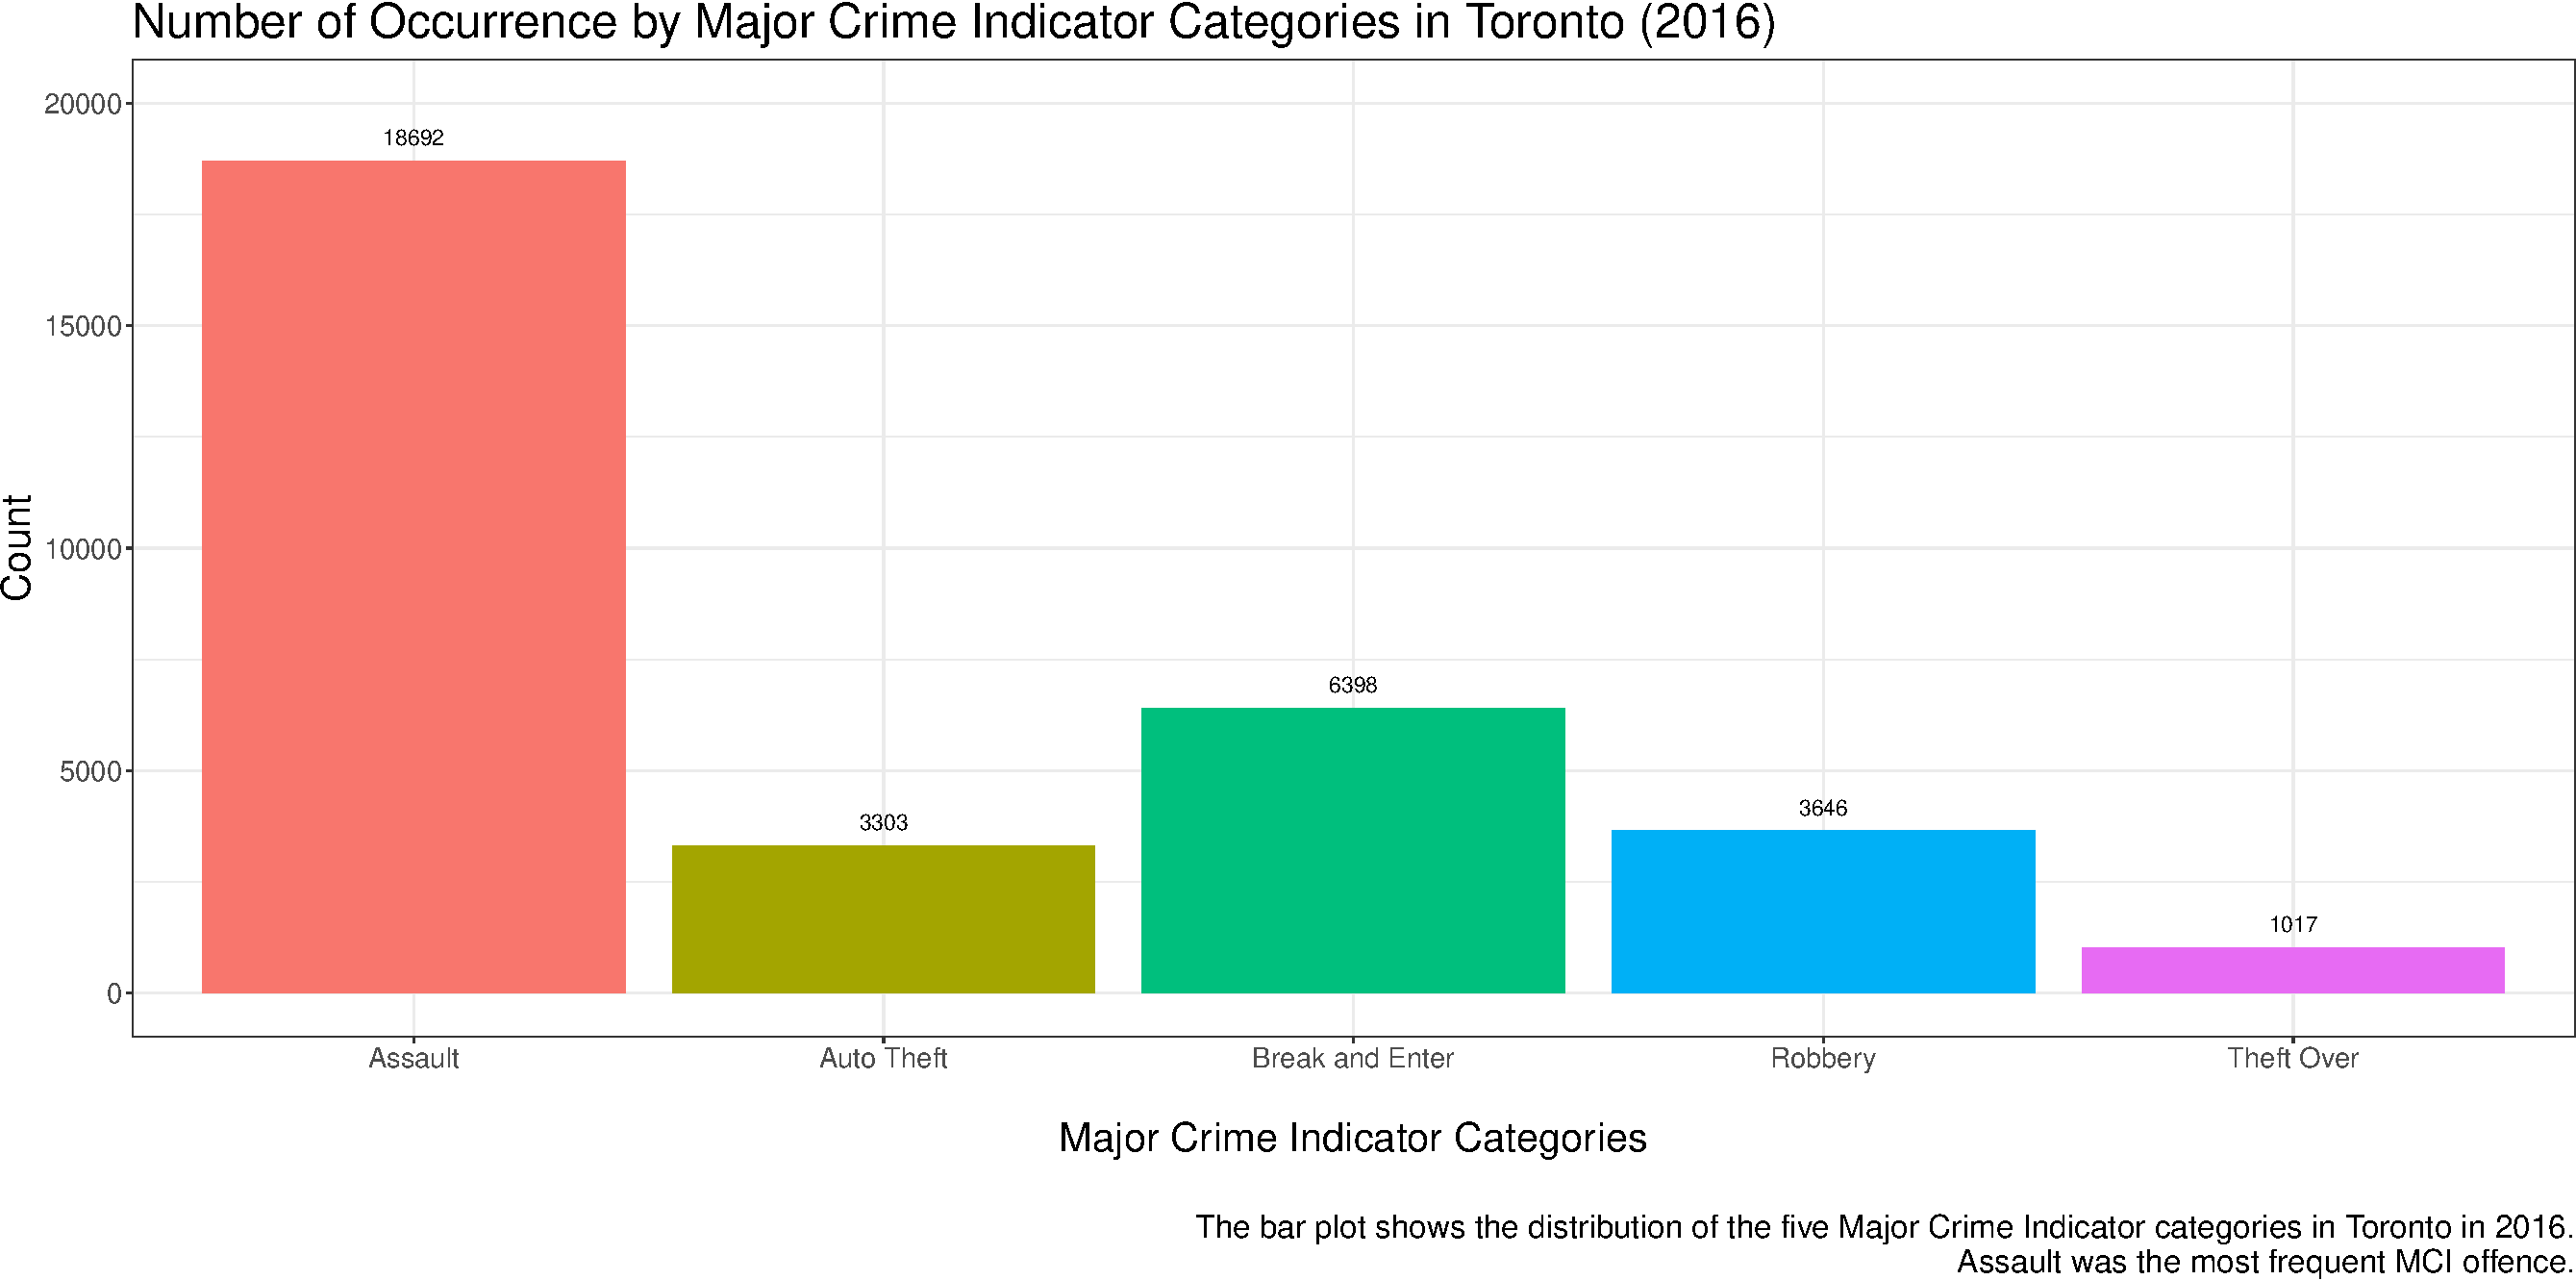
\includegraphics{Midterm-Report_files/figure-latex/crime-count-1.pdf}

To inspect where these major crimes occurred, two stacked bar plots were
created, which showed the distribution of crime occurrences and where
they occurred. From these plots, there were some interesting
observations: first, ``assault'' was the predominant crime in the seven
premises type shown below, especially in Transit where it was about
seven times more likely to occur than all the other four crimes. This
suggested that neighbourhoods with large transit hubs were more likely
to suffer from assault offences, or neighbourhoods with a higher
population density; second, nearly half of the ``auto theft'' offences
occurred outside. This suggested that neighbourhoods with more indoor or
underground parking spaces might be less susceptible to auto theft;
third, the number of crimes occurred in houses were about 80\% of that
in apartments, but assuming that apartments usually house many more
people than a house could, this suggested that the number of offences
per person might be higher in houses (which appear in less busy areas)
than apartments (which are often in city centers).

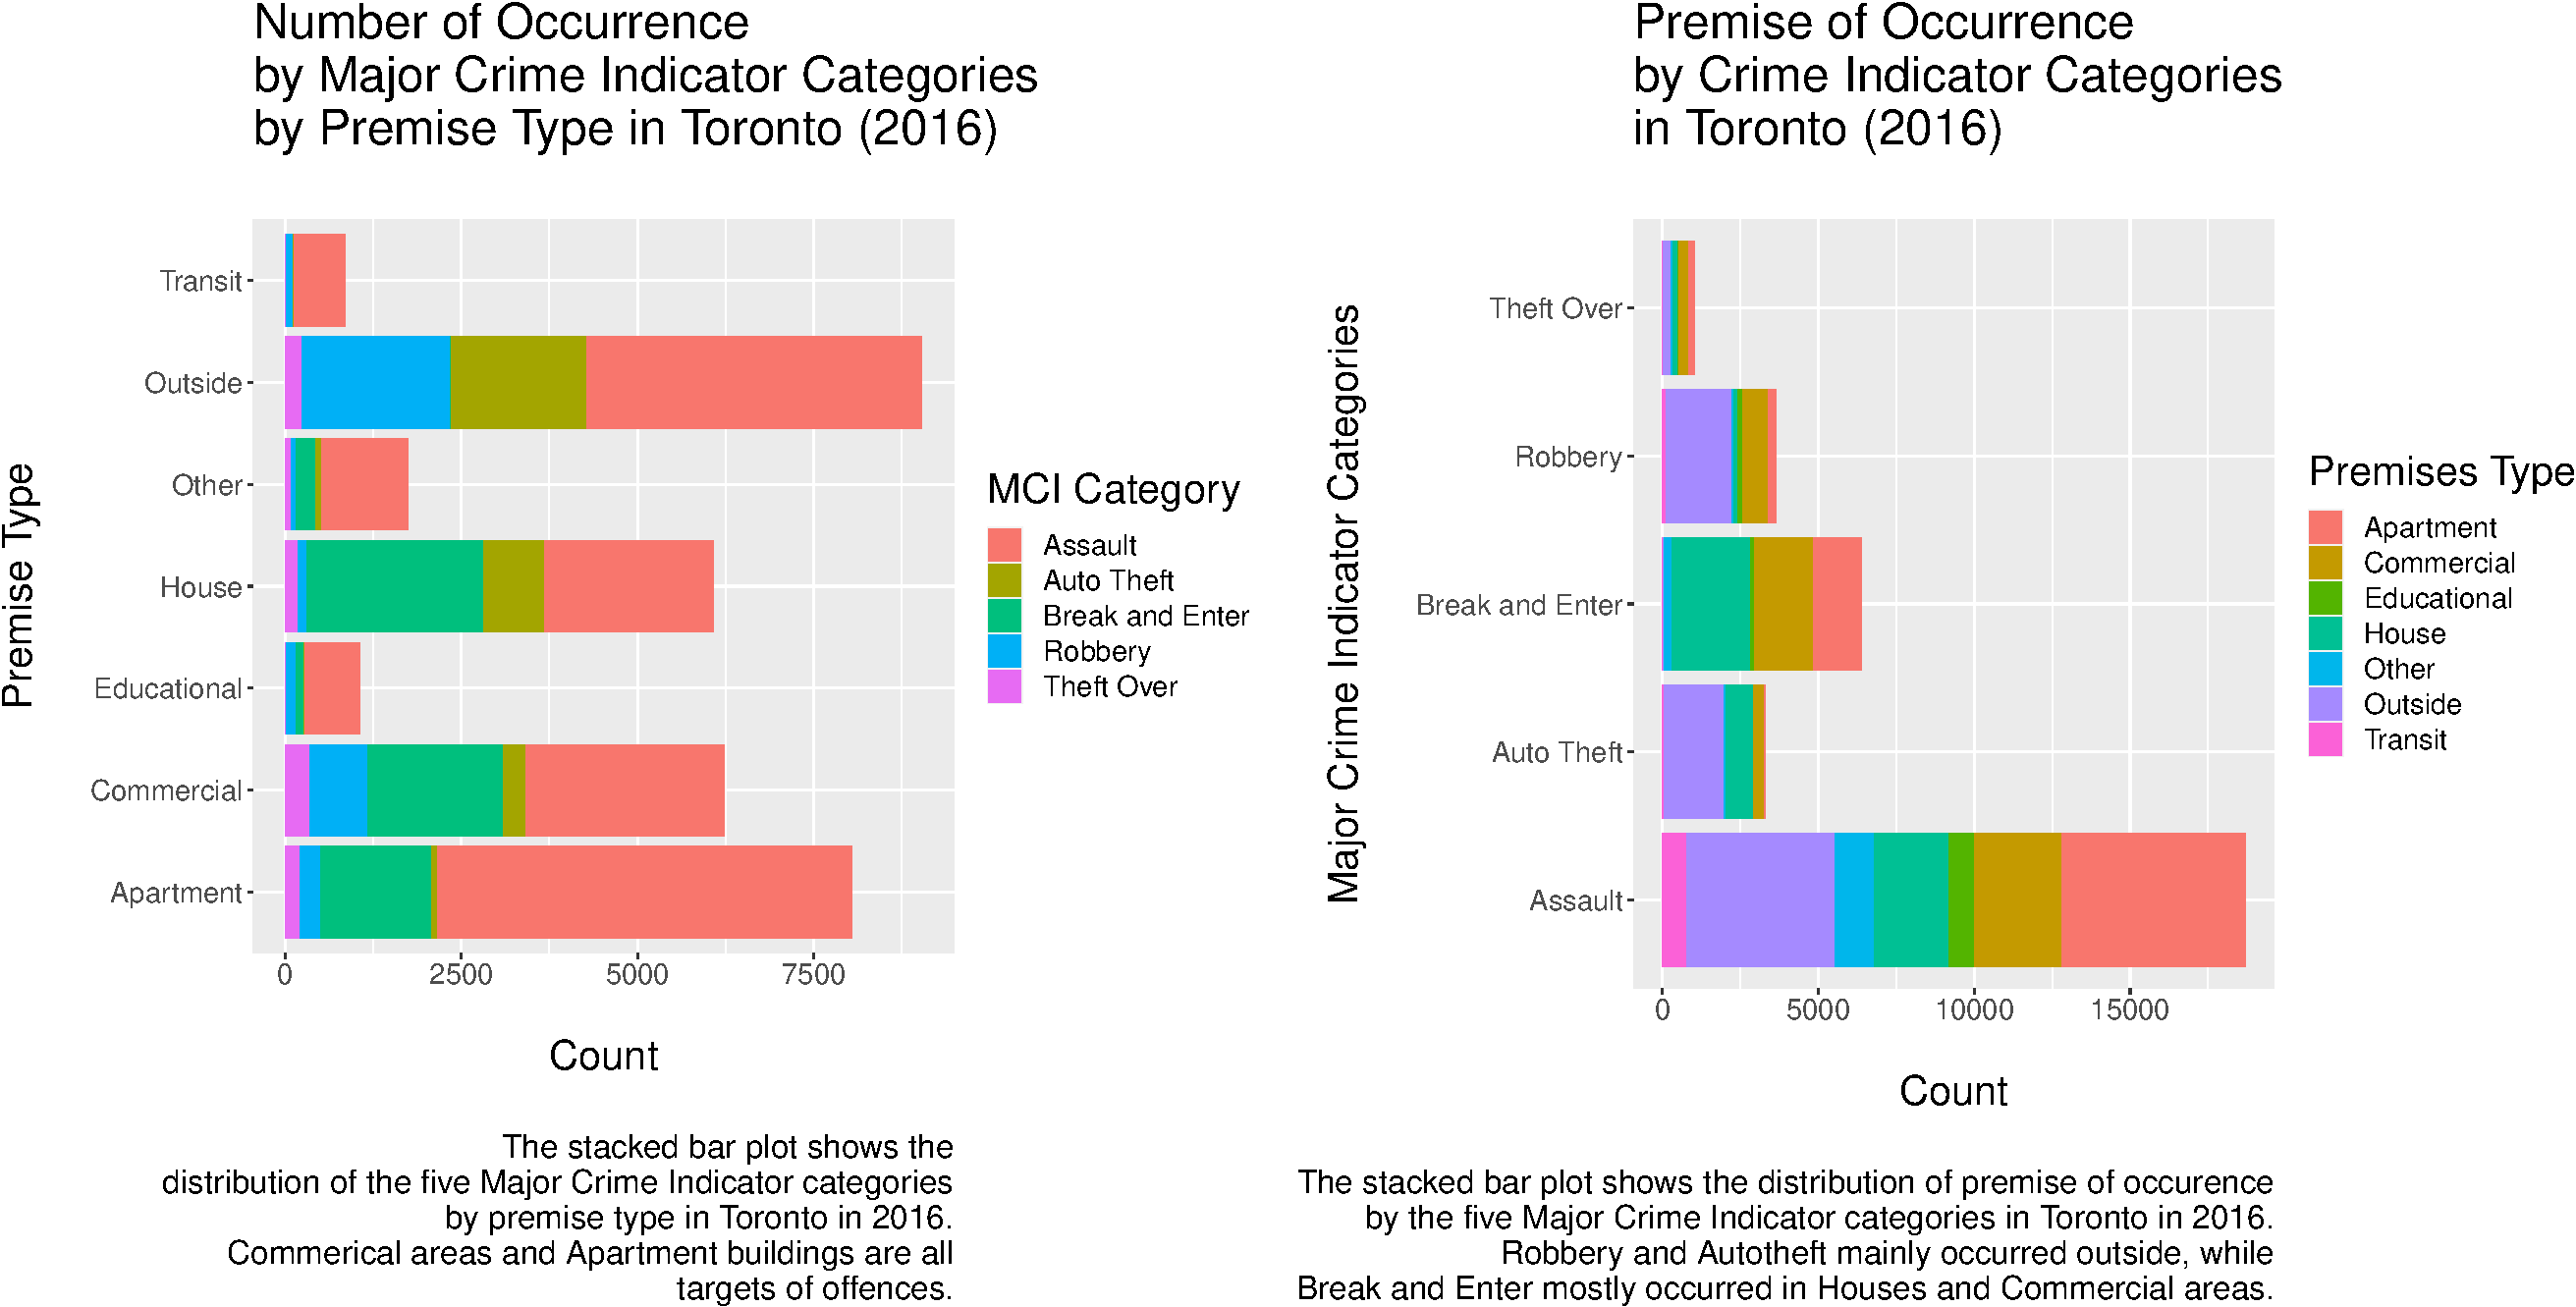
\includegraphics{Midterm-Report_files/figure-latex/crime-count-by-premise-1.pdf}

We also inspected the trend of offence occurrences with respect to time
in 2016 with the histogram below. The trend shown in the plot suggests
that there were no significant relationship between the day of year and
the number of major crime occurred, as the plot appears to be close to a
uniform distribution with only minor fluctuations periodically. The
spike at Day 0 is due to the fact the some data with missing date were
marked with 0, but these were kept in our cleaned data since we cared
more about the number of occurrences instead of crimes at a specific
date.

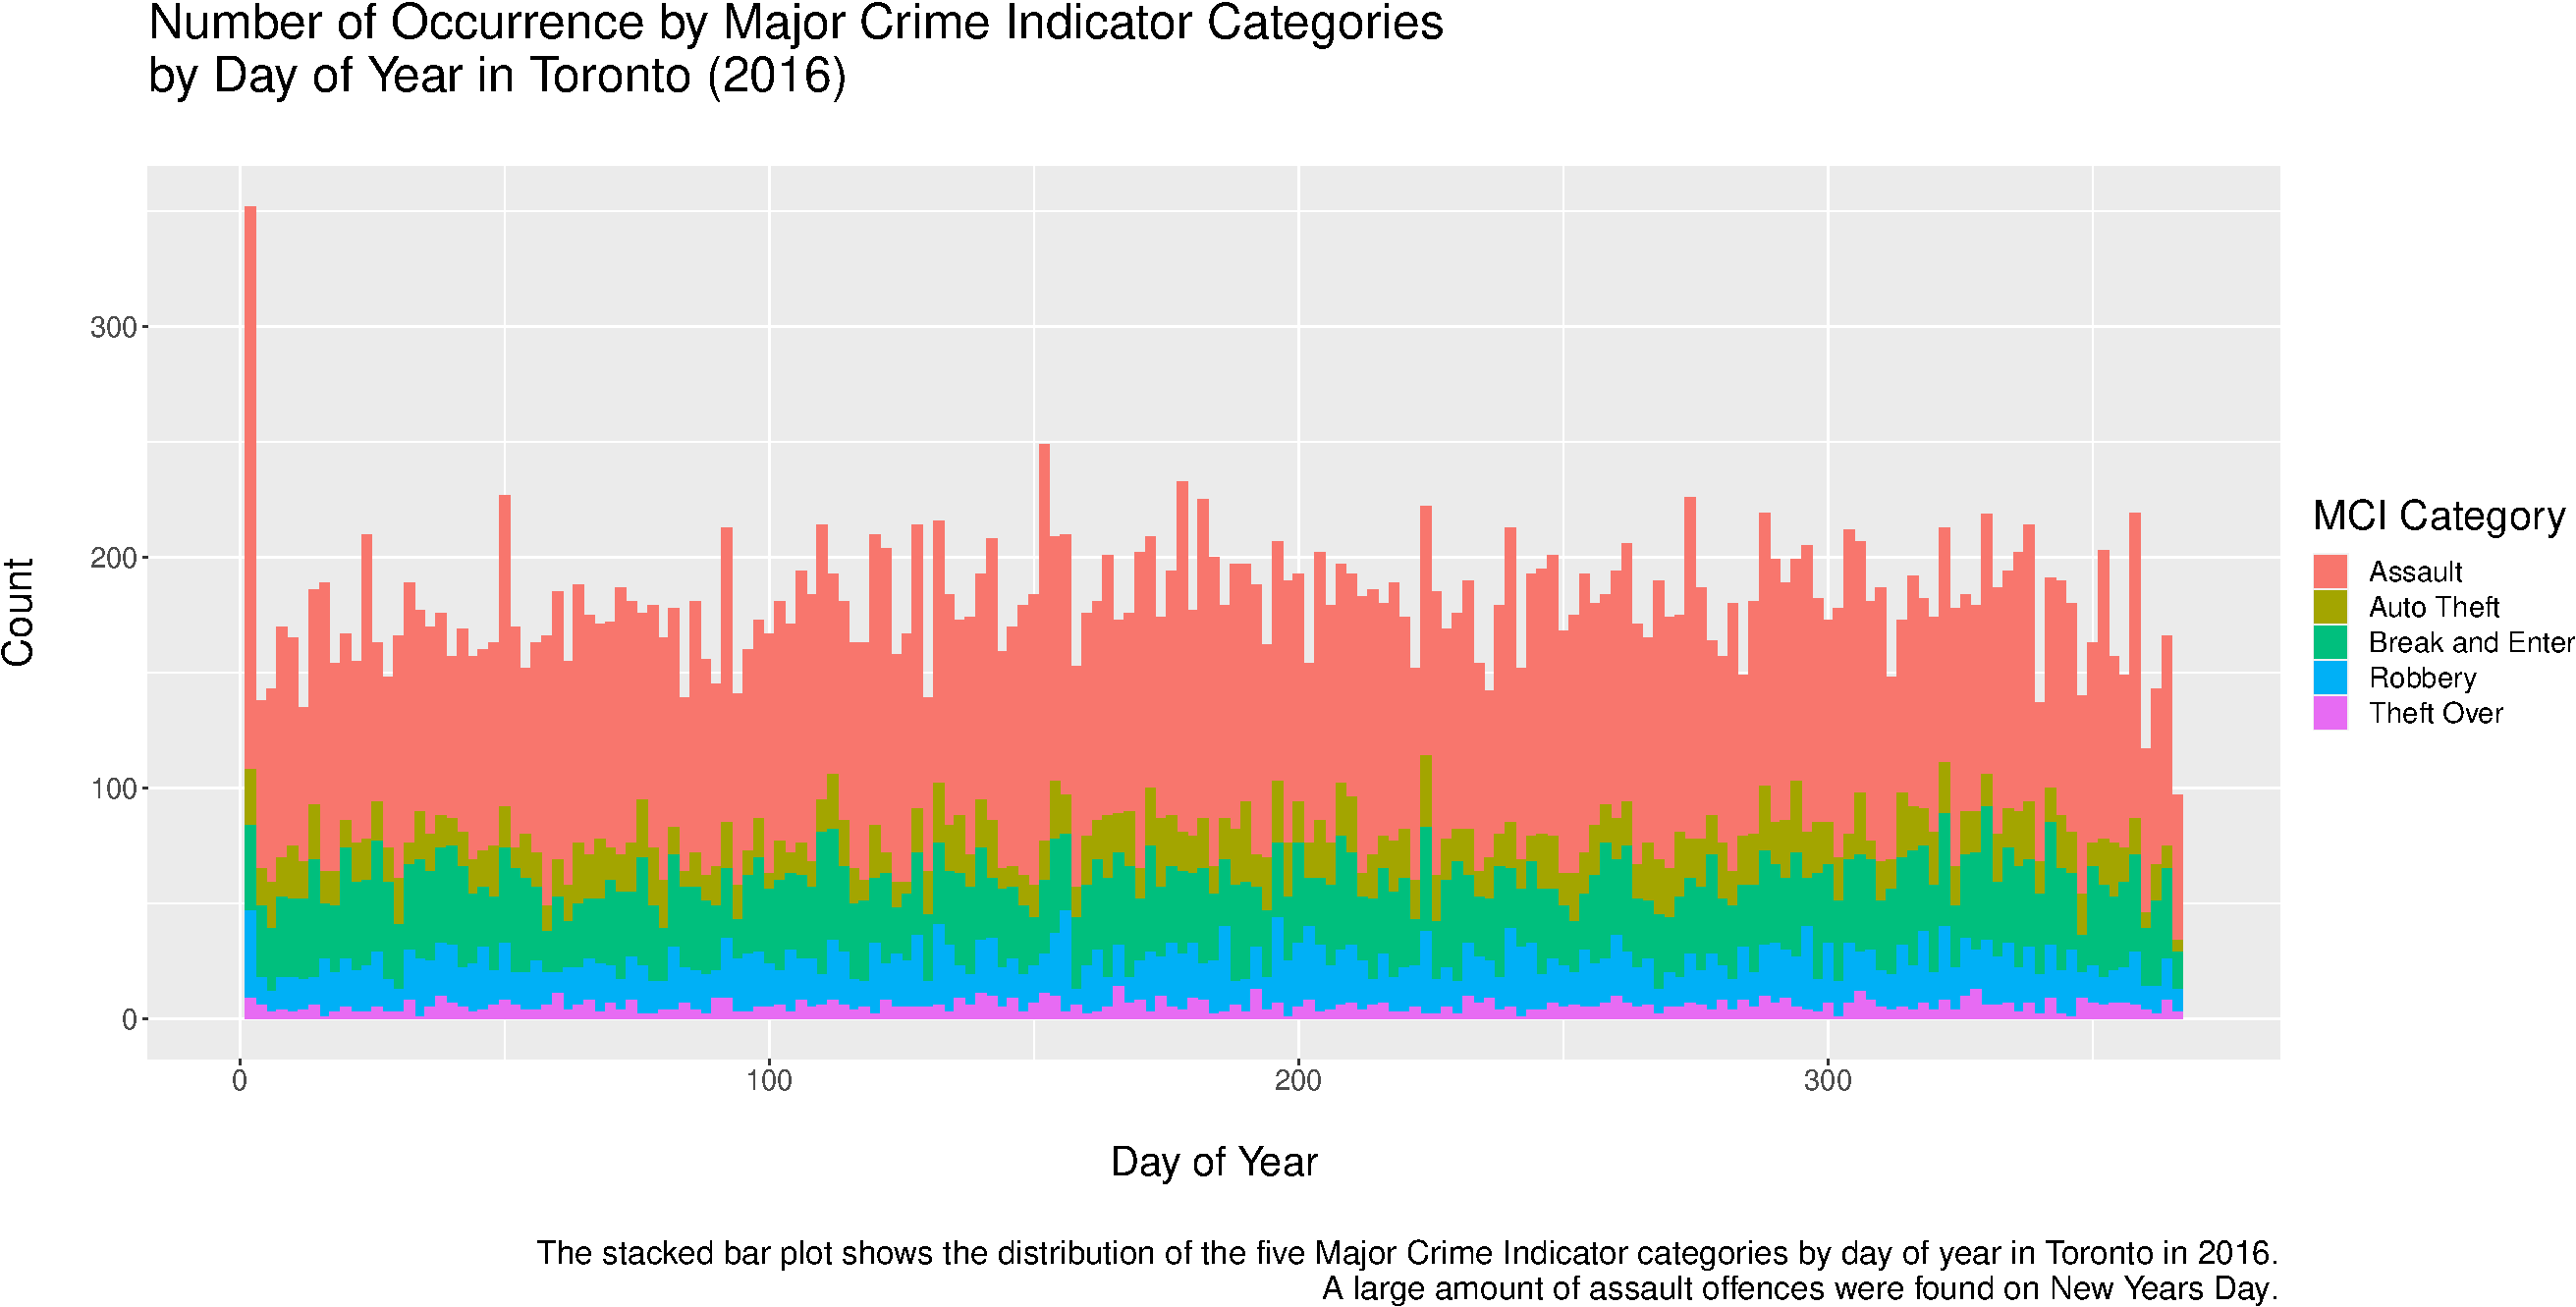
\includegraphics{Midterm-Report_files/figure-latex/crime-by-time-1.pdf}

The following barplot shows the Top 10 Neighbourhoods sorted by the
number of major crime occurrences in 2016 in descending order. The
results did not come as surprising, as the neighbourhood with the most
population (Waterfront Communities Population: 65913) had the highest
crime occurrences. Busy city centres were also in the plot (Bay Street,
Church-Yonge). Interestingly, West Humber Clairville had significantly
more auto theft offences compared to the other neighbourhoods, which was
80\% of all the other 9 neighbourhoods combined (318 vs 385).

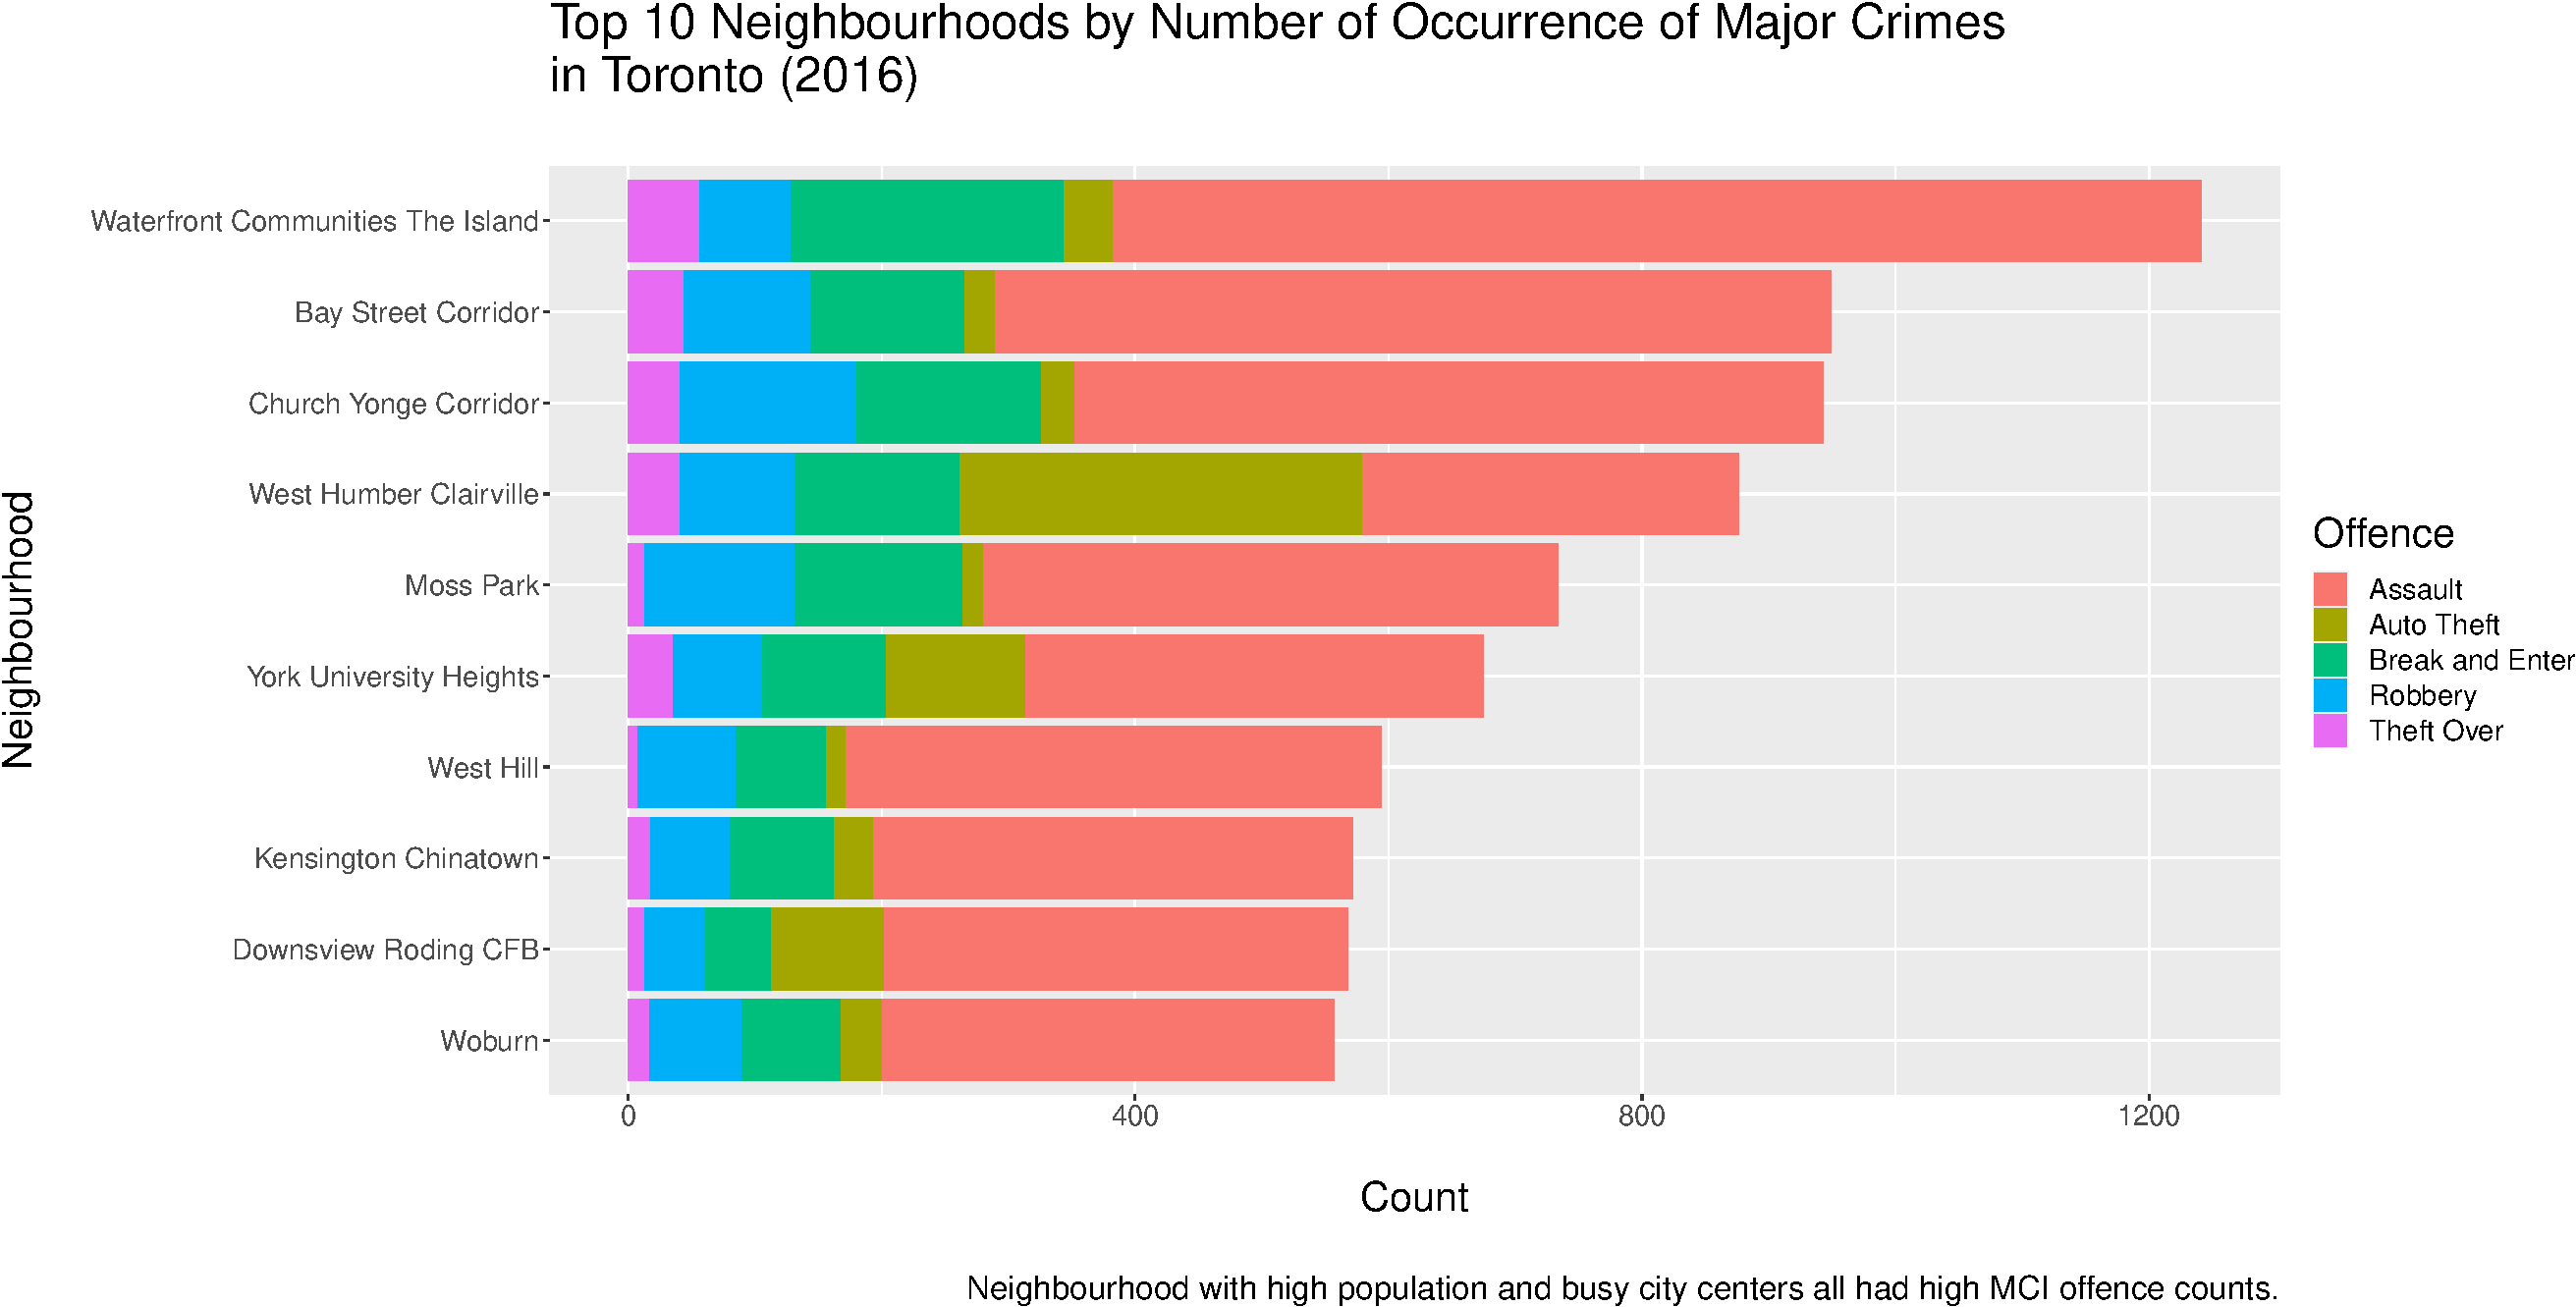
\includegraphics{Midterm-Report_files/figure-latex/crime-by-neighbourhood-1.pdf}

We also plotted an interactive heat map of number of MCI offences per
neighbourhood. To access the interactive widget, extract crime\_map.html
and the directory crime\_map\_files and place them in the same
directory. Then click and open crime\_map.html.

The crime map shows the distribution of MCI offences in the 140
offences, filtered by offence type and total count. From the heatmap, we
could see that areas which were further away from city centers and urban
areas had lower number of reported offences.

\hypertarget{preliminary-results}{%
\section{Preliminary Results}\label{preliminary-results}}

We inspected the relationship between the crime rate and the variables
of interests, i.e.~population size, population age, education,
employment/labour, immigration and citizenship status, income taxes, and
the level of visible minority. For each variable, we already extracted
the sub-table which contained only the relevant fields from the original
dataset in the ``Data Cleaning'' section. For each of these sub-tables,
we merged them with the table containing (Neighbourhood, Population)
tuples, and further merged them with the table containing the number of
reported crime per offence type.

\hypertarget{relationship-between-population-size-and-crime-rate}{%
\subsection{Relationship between Population Size and Crime
Rate}\label{relationship-between-population-size-and-crime-rate}}

It is not surprising that the best fitted lines shows that the number of
offences increases with the number of population in a neighbourhood.
However, in all the subplots, the majority of the neighbourhoods had a
population of less than 30 thousand, and there are outliers and
influential points in the plots. A better indicator of crime rate versus
population might be plotting the crime rate against the population
density instead, which is more representative of the scale of crime rate
in terms of neighbourhood size: a neighbourhood with higher population
density is more likely to have higher crime rate.

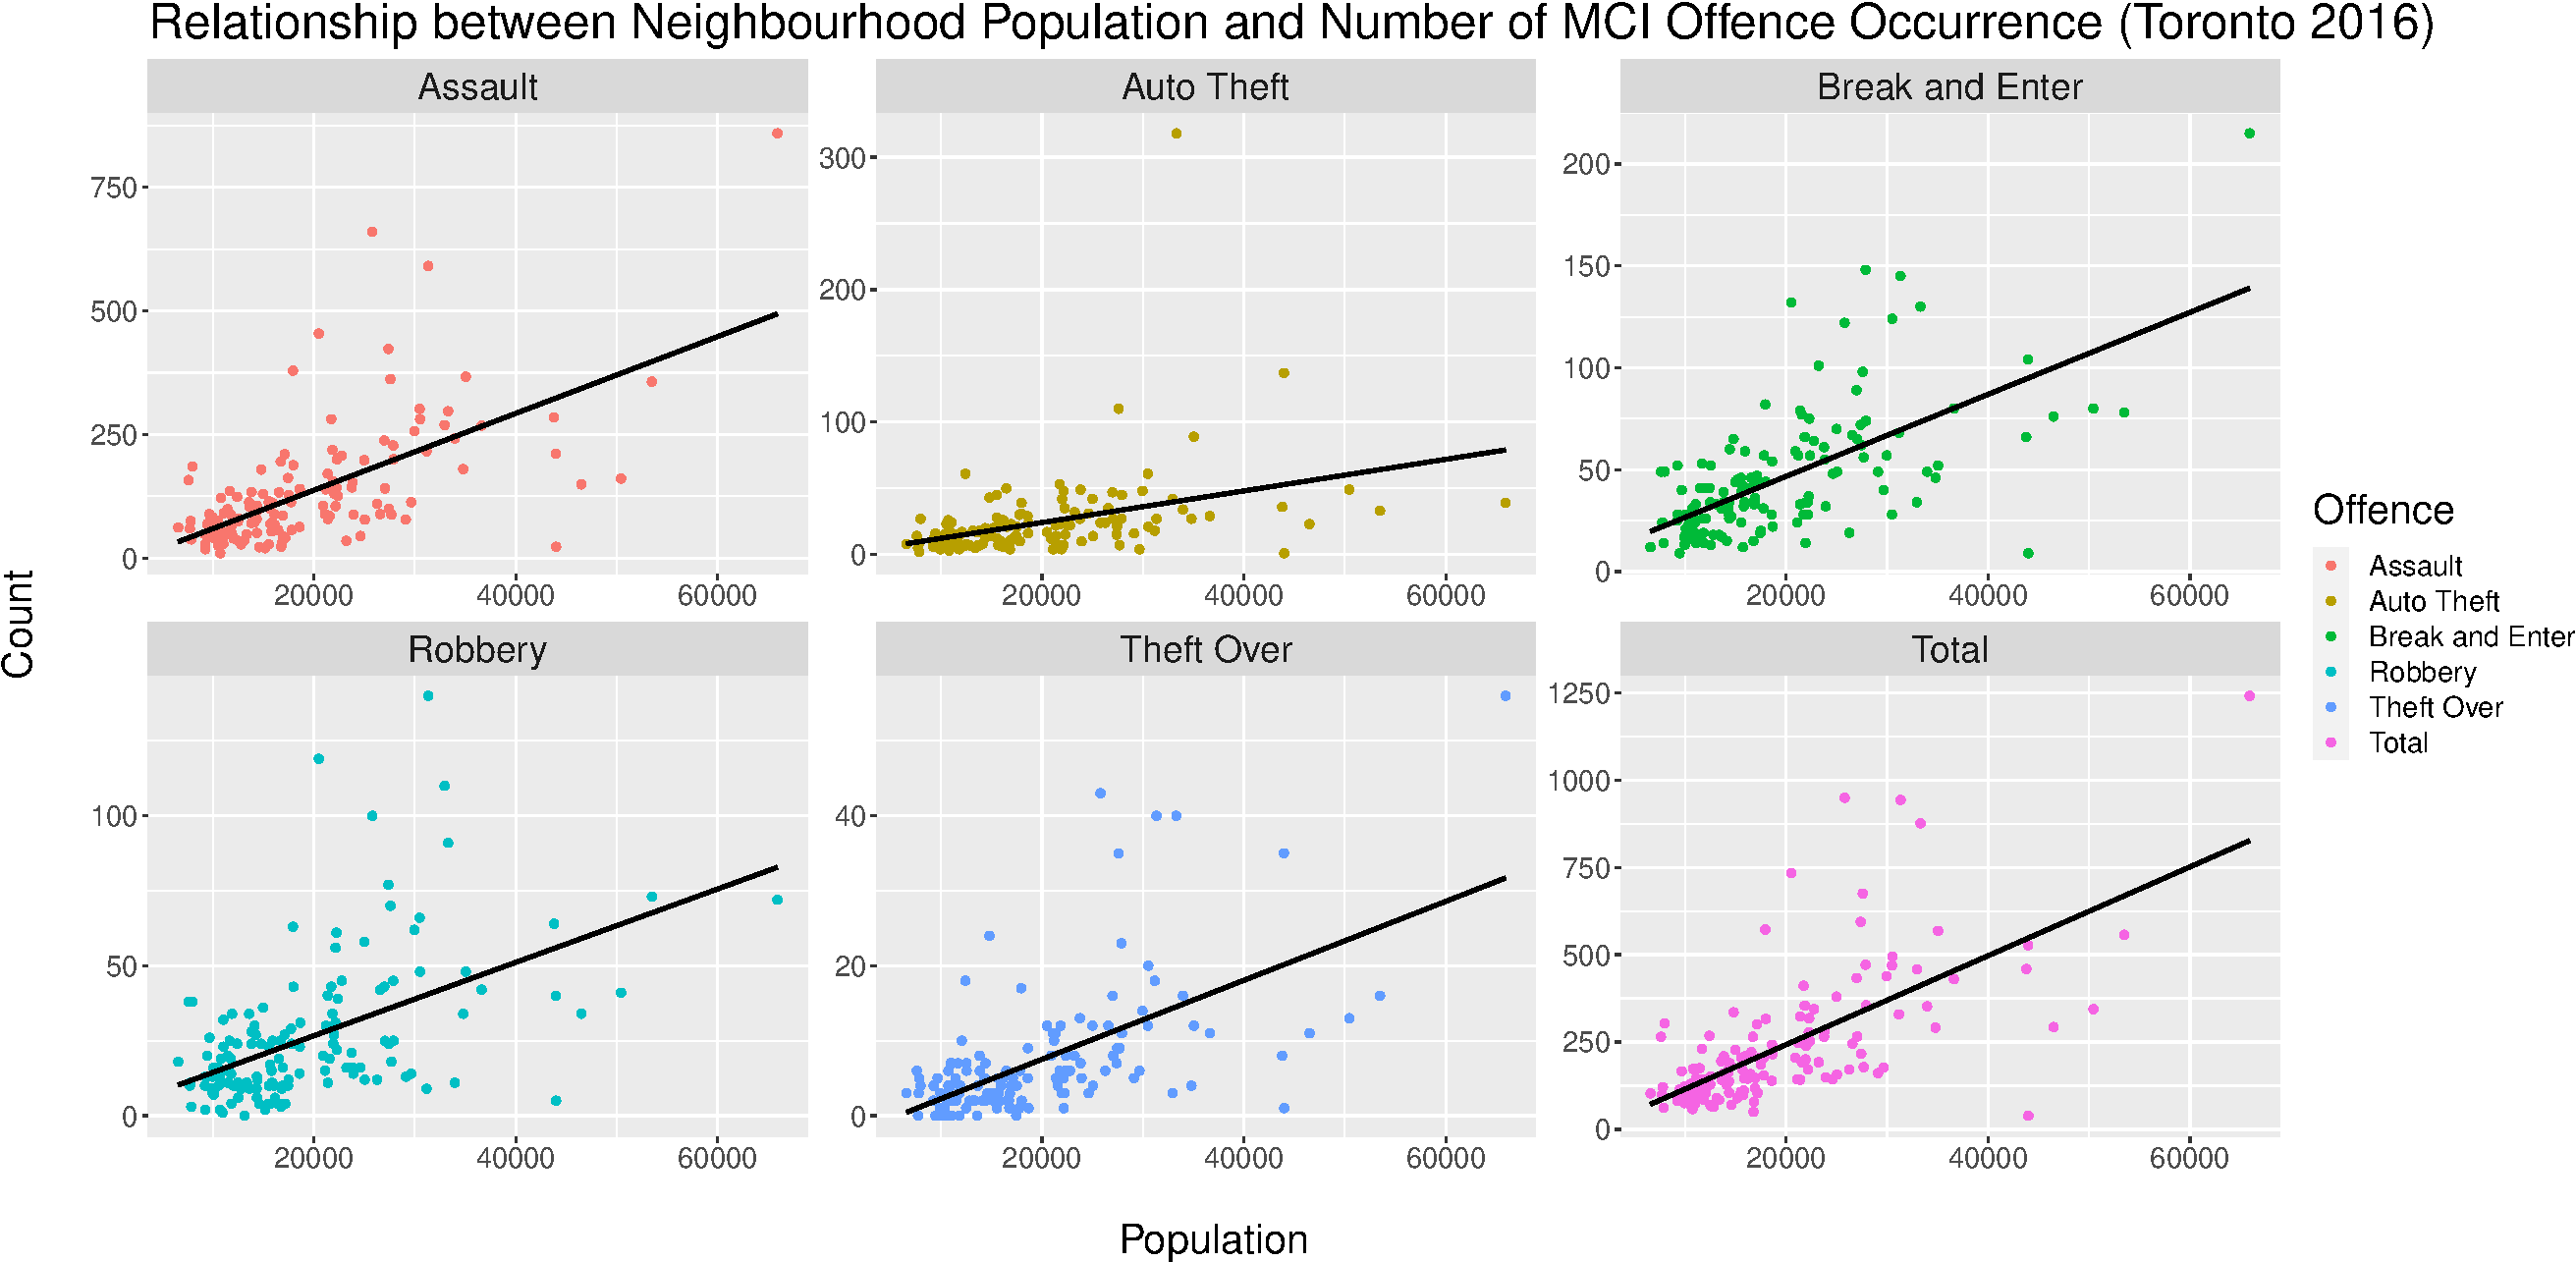
\includegraphics{Midterm-Report_files/figure-latex/crime-vs-population-2-1.pdf}

\hypertarget{relationship-between-population-age-and-crime-rate}{%
\subsection{Relationship between Population Age and Crime
Rate}\label{relationship-between-population-age-and-crime-rate}}

We fitted a basic linear model where the response variable was the
number of offences and the variables were the proportion of different
age groups in the neighbourhood. Note that in the original dataset,
there were two additional age groups (Seniors (65+ years) and Older
Seniors (85+ years)). However, we did not include them in this
preliminary model as it would induce multicollinearity, since these
proportions of age groups add up to 1.

From the p-values below, we can see that the proportion of age groups
are all statistically significant. Based on the signs of the estimated
coefficients, they confirm from our previous findings that a
neighbourhood with larger proportion of senior residents are likely to
have fewer crime rate (negative coefficient), while increasing number of
youths (positive coefficient) is more likely to the crime
rate\footnote{Ulmer, J. T., \& Steffensmeier, D. (2014). The age and
  crime relationship: Social variation, social explanations. In The
  Nurture Versus Biosocial Debate in Criminology: On the Origins of
  Criminal Behavior and Criminality (pp.~377-396). SAGE Publications
  Inc.. \url{https://doi.org/10.4135/9781483349114.n23}}.

\begin{longtable}[]{@{}
  >{\raggedright\arraybackslash}p{(\columnwidth - 8\tabcolsep) * \real{0.4627}}
  >{\raggedleft\arraybackslash}p{(\columnwidth - 8\tabcolsep) * \real{0.1343}}
  >{\raggedleft\arraybackslash}p{(\columnwidth - 8\tabcolsep) * \real{0.1642}}
  >{\raggedleft\arraybackslash}p{(\columnwidth - 8\tabcolsep) * \real{0.1194}}
  >{\raggedleft\arraybackslash}p{(\columnwidth - 8\tabcolsep) * \real{0.1194}}@{}}
\caption{Coefficient Estimates of a Linear Regression Model for
Estimating MCI Offence Count (Age Groups)}\tabularnewline
\toprule()
\begin{minipage}[b]{\linewidth}\raggedright
Terms
\end{minipage} & \begin{minipage}[b]{\linewidth}\raggedleft
Estimate
\end{minipage} & \begin{minipage}[b]{\linewidth}\raggedleft
Std. Error
\end{minipage} & \begin{minipage}[b]{\linewidth}\raggedleft
t-value
\end{minipage} & \begin{minipage}[b]{\linewidth}\raggedleft
p-value
\end{minipage} \\
\midrule()
\endfirsthead
\toprule()
\begin{minipage}[b]{\linewidth}\raggedright
Terms
\end{minipage} & \begin{minipage}[b]{\linewidth}\raggedleft
Estimate
\end{minipage} & \begin{minipage}[b]{\linewidth}\raggedleft
Std. Error
\end{minipage} & \begin{minipage}[b]{\linewidth}\raggedleft
t-value
\end{minipage} & \begin{minipage}[b]{\linewidth}\raggedleft
p-value
\end{minipage} \\
\midrule()
\endhead
(Intercept) & 57.993 & 21.730 & 2.669 & 0.009 \\
\texttt{Children\ (0-14\ years)} & -0.032 & 0.012 & -2.660 & 0.009 \\
\texttt{Youth\ (15-24\ years)} & 0.125 & 0.015 & 8.320 & 0.000 \\
\texttt{Working\ Age\ (25-54\ years)} & 0.014 & 0.003 & 4.286 & 0.000 \\
\texttt{Pre-retirement\ (55-64\ years)} & -0.065 & 0.019 & -3.351 &
0.001 \\
\bottomrule()
\end{longtable}

\hypertarget{relationship-between-education-and-crime-rate}{%
\subsection{Relationship between Education and Crime
Rate}\label{relationship-between-education-and-crime-rate}}

We also fitted a basic linear model where the response variable is the
number of MCI offences and the predictors are the proprtion of people
with different levels of education. From the summary, we can see that an
increase proportion of people with secondary and postsecondary education
increases the number of crime rates, but the increase is around 3 times
as big for an increase in proportion of people with only secondary
education than those with postsecondary education. Again, we did not
include the group No certificate, diploma or degree in this preliminary
model as it would induce multicollinearity.

\begin{longtable}[]{@{}
  >{\raggedright\arraybackslash}p{(\columnwidth - 8\tabcolsep) * \real{0.6364}}
  >{\raggedleft\arraybackslash}p{(\columnwidth - 8\tabcolsep) * \real{0.0909}}
  >{\raggedleft\arraybackslash}p{(\columnwidth - 8\tabcolsep) * \real{0.1111}}
  >{\raggedleft\arraybackslash}p{(\columnwidth - 8\tabcolsep) * \real{0.0808}}
  >{\raggedleft\arraybackslash}p{(\columnwidth - 8\tabcolsep) * \real{0.0808}}@{}}
\caption{Coefficient Estimates of a Linear Regression Model for
Estimating MCI Offence Count (Education)}\tabularnewline
\toprule()
\begin{minipage}[b]{\linewidth}\raggedright
Terms
\end{minipage} & \begin{minipage}[b]{\linewidth}\raggedleft
Estimate
\end{minipage} & \begin{minipage}[b]{\linewidth}\raggedleft
Std. Error
\end{minipage} & \begin{minipage}[b]{\linewidth}\raggedleft
t-value
\end{minipage} & \begin{minipage}[b]{\linewidth}\raggedleft
p-value
\end{minipage} \\
\midrule()
\endfirsthead
\toprule()
\begin{minipage}[b]{\linewidth}\raggedright
Terms
\end{minipage} & \begin{minipage}[b]{\linewidth}\raggedleft
Estimate
\end{minipage} & \begin{minipage}[b]{\linewidth}\raggedleft
Std. Error
\end{minipage} & \begin{minipage}[b]{\linewidth}\raggedleft
t-value
\end{minipage} & \begin{minipage}[b]{\linewidth}\raggedleft
p-value
\end{minipage} \\
\midrule()
\endhead
(Intercept) & -581.034 & 256.482 & -2.265 & 0.025 \\
\texttt{Postsecondary\ certificate,\ diploma\ or\ degree} & 708.739 &
250.138 & 2.833 & 0.005 \\
\texttt{Secondary\ (high)\ school\ diploma\ or\ equivalency\ certificate}
& 2299.184 & 711.735 & 3.230 & 0.002 \\
\bottomrule()
\end{longtable}

\hypertarget{relationship-between-employment-and-crime-rate}{%
\subsection{Relationship between Employment and Crime
Rate}\label{relationship-between-employment-and-crime-rate}}

The fitted linear model below shows that the effect of the number of
people who did not work in a neighbourhood on crime rate was
statistically significant. This result aligned with the common consensus
that unemployment rate was positively correlated with crime rate
(Farrington et al.~1986\footnote{Farrington, D. P., Gallagher, B.,
  Morley, L., St.~Ledger, R. J., \& West, D. J. (1986). UNEMPLOYMENT,
  SCHOOL LEAVING, AND CRIME. The British Journal of Criminology, 26(4),
  335--356. \url{http://www.jstor.org/stable/23637076}}, John Howard
Society of Ontario 2009\footnote{\url{https://johnhoward.on.ca/wp-content/uploads/2014/09/facts-24-crime-and-unemployment-whats-the-link-march-2009.pdf}}).

\begin{longtable}[]{@{}lrrrr@{}}
\caption{Coefficient Estimates of a Linear Regression Model for
Estimating MCI Offence Count (Employment Status)}\tabularnewline
\toprule()
Terms & Estimate & Std. Error & t-value & p-value \\
\midrule()
\endfirsthead
\toprule()
Terms & Estimate & Std. Error & t-value & p-value \\
\midrule()
\endhead
(Intercept) & 57.258 & 28.187 & 2.031 & 0.044 \\
\texttt{Did\ not\ work} & 0.032 & 0.004 & 7.282 & 0.000 \\
\bottomrule()
\end{longtable}

\hypertarget{relationship-between-immigration-and-citizenship-status-and-crime-rate}{%
\subsection{Relationship between Immigration and Citizenship Status and
Crime
Rate}\label{relationship-between-immigration-and-citizenship-status-and-crime-rate}}

We plotted the number of MCI offences against the proprtion of
immigrants in the 140 neighbourhoods, separated by offence type and also
included a total count. From these plots, we can see that as the
proportion of immigrants increased in a neighbourhood, the number of
crimes committed decreases, with the exception of ``Break and Enter''
which stayed roughly the same. This aligned with our prior findings
which concluded that the number of immigrants
(statistically-)significantly reduced the number of crimes in the
area\footnote{Statistics Canada. (n.d.). Main article. Neighbourhood
  Characteristics and the Distribution of Police-reported Crime in the
  City of Toronto. Retrieved March 13, 2023, from
  \url{https://www150.statcan.gc.ca/n1/pub/85-561-m/2009018/part-partie1-eng.htm}}.

\begin{longtable}[]{@{}lrrrr@{}}
\caption{Coefficient Estimates of a Linear Regression Model for
Estimating MCI Offence Count (Employment Status)}\tabularnewline
\toprule()
Terms & Estimate & Std. Error & t-value & p-value \\
\midrule()
\endfirsthead
\toprule()
Terms & Estimate & Std. Error & t-value & p-value \\
\midrule()
\endhead
(Intercept) & 378.555 & 59.861 & 6.324 & 0.000 \\
Immigration\_Rate & -278.403 & 112.786 & -2.468 & 0.015 \\
\bottomrule()
\end{longtable}

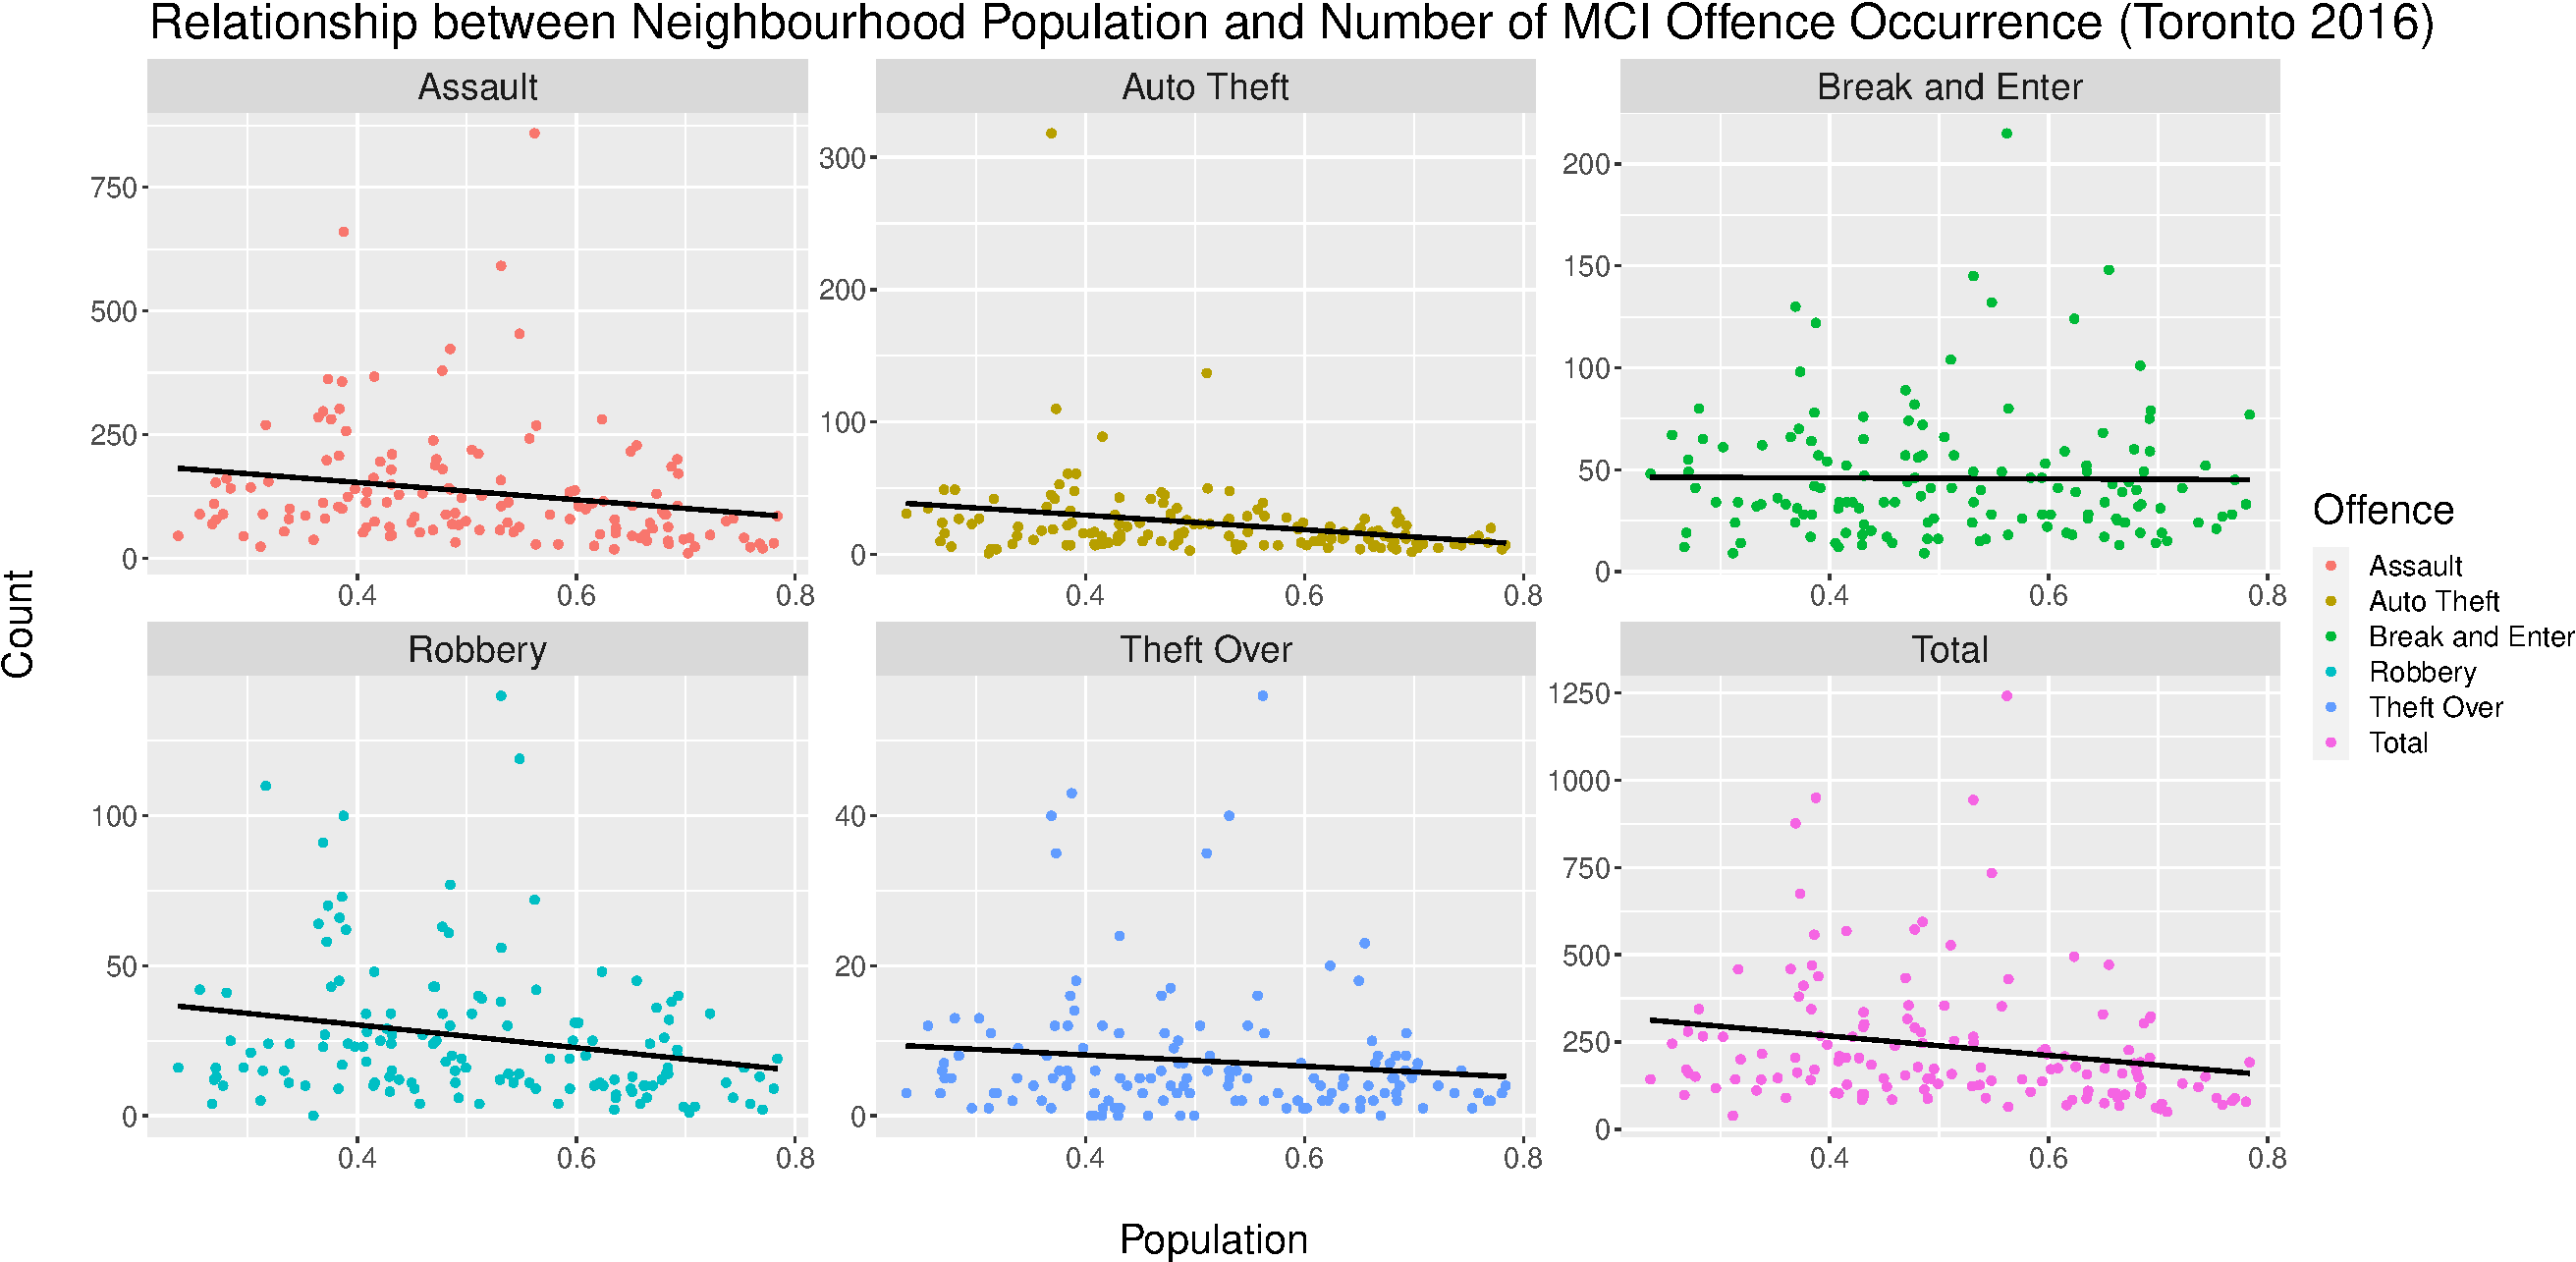
\includegraphics{Midterm-Report_files/figure-latex/crime-vs-immigration-lm-1.pdf}

\hypertarget{relationship-between-visible-minority-and-crime-rate}{%
\subsection{Relationship between Visible Minority and Crime
Rate}\label{relationship-between-visible-minority-and-crime-rate}}

A racially-diversed neighbourhood were found to be linked to lower crime
rate, especially in rural areas\footnote{Kim, Y.-A., \& Wo, J. C. (2022,
  April 1). Racially diverse neighborhoods in diverse areas are linked
  to lower crime rates. Racially diverse neighborhoods in diverse areas
  are linked to lower crime rates Comments. Retrieved March 13, 2023,
  from
  \url{https://blogs.lse.ac.uk/usappblog/2022/04/01/racially-diverse-neighborhoods-in-diverse-areas-are-linked-to-lower-crime-rates/}}.
Hence, we chose to explore the relationship of neighbourhood crime rate
and the proportion of visible minority because we believed that this
feature was also related to immigration and citizenship status, which
was found to be correlated with crime rate\footnote{Statistics Canada.
  (n.d.). Main article. Neighbourhood Characteristics and the
  Distribution of Police-reported Crime in the City of Toronto.
  Retrieved March 13, 2023, from
  \url{https://www150.statcan.gc.ca/n1/pub/85-561-m/2009018/part-partie1-eng.htm}}.
However, unlike the number of immigrants, we could see that crime rates
were likely to be weakly positively correlated with the proportion of
visible minority in the neighbourhood from the plots. The number of
outliers in the plots might suggest why we obtained a different result
than expected.

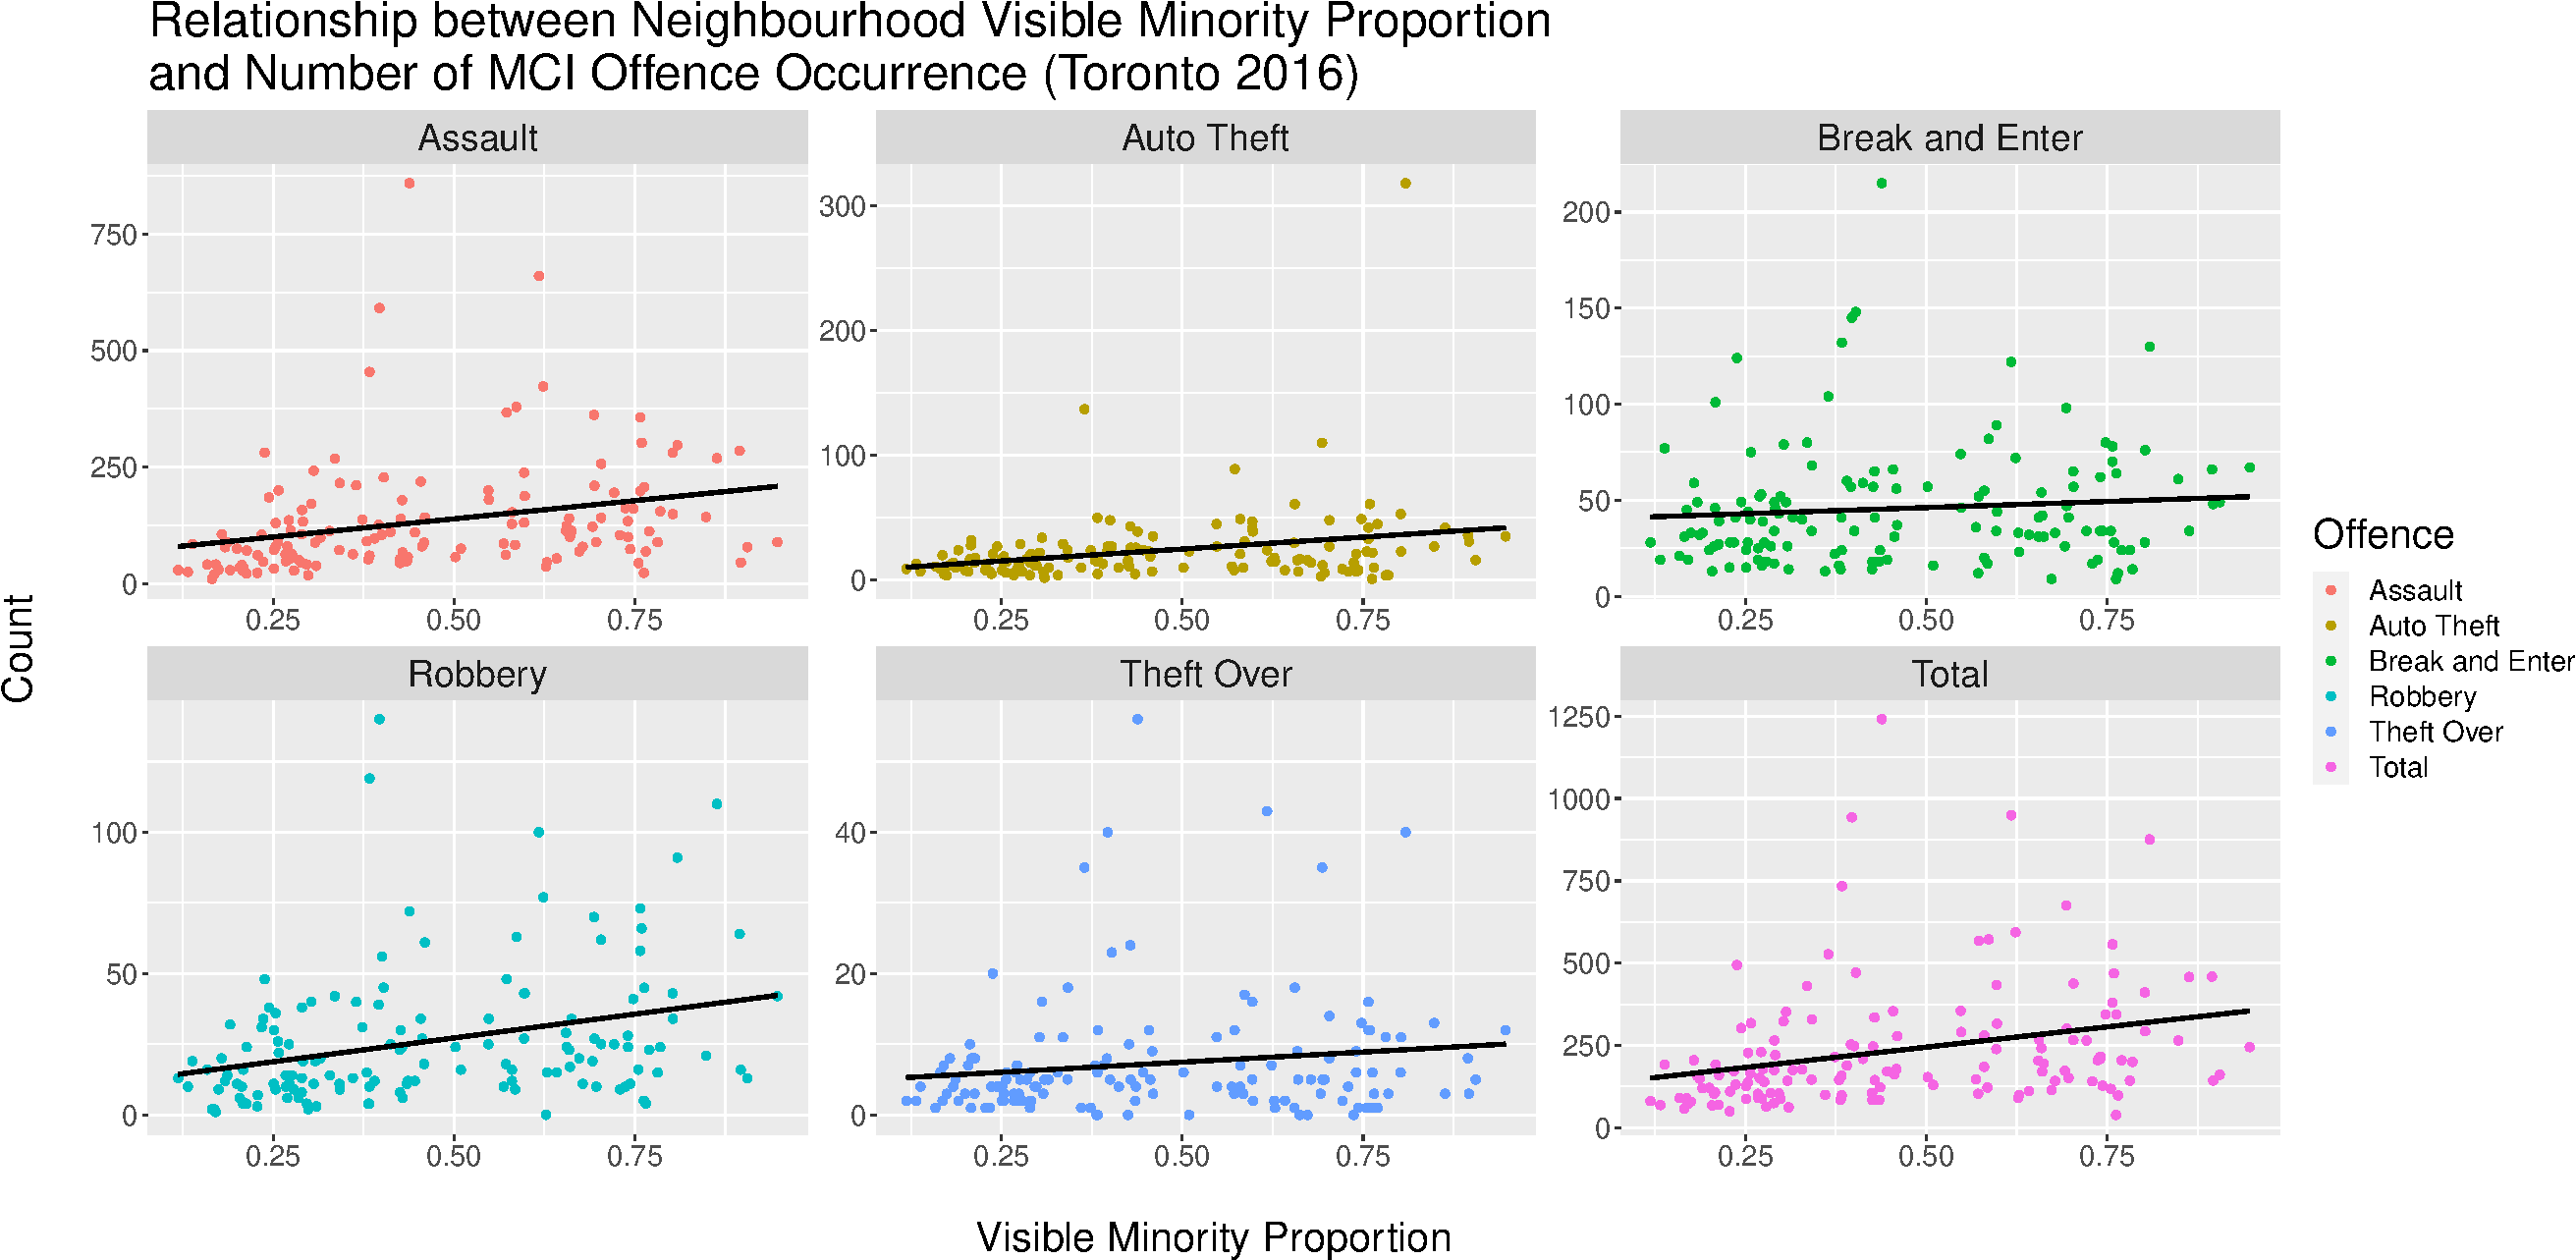
\includegraphics{Midterm-Report_files/figure-latex/crime-vs-minority-plot-1.pdf}

\hypertarget{relationship-between-income-and-crime-rate}{%
\subsection{Relationship between Income and Crime
Rate}\label{relationship-between-income-and-crime-rate}}

To estimate the effect of average individual income on a neighbourhood's
crime rate, we plotted the number of offences against average income tax
per offence type. From the data cleaning process, the data for income
groups were corrupted (see Data Cleaning section about ``data
indentation''). Thus, we decided to use the average income tax as an
indicator of household income level for each neighbourhood. From the six
subplots, we can see that the number of all offence types decrease as
the average income tax of the neighbourhood increases, with the
exception of ``Break and Enter''. This does not come as surprising as
wealthy neighbourhoods were more likely to have better security, and
relative risk associated with theft in wealthy neighbourhoods
outweighted the possibility of stealing more expensive goods, which
possibly deterred thefts in these areas\footnote{Chamberlain, A. W., \&
  Boggess, L. N. (2016, September 26). Why disadvantaged neighborhoods
  are more attractive targets for burgling than wealthy ones. Why
  disadvantaged neighborhoods are more attractive targets for burgling
  than wealthy ones Comments. Retrieved March 13, 2023, from
  \url{https://blogs.lse.ac.uk/usappblog/2016/09/26/why-disadvantaged-neighborhoods-are-more-attractive-targets-for-burgling-than-wealthy-ones/}}.

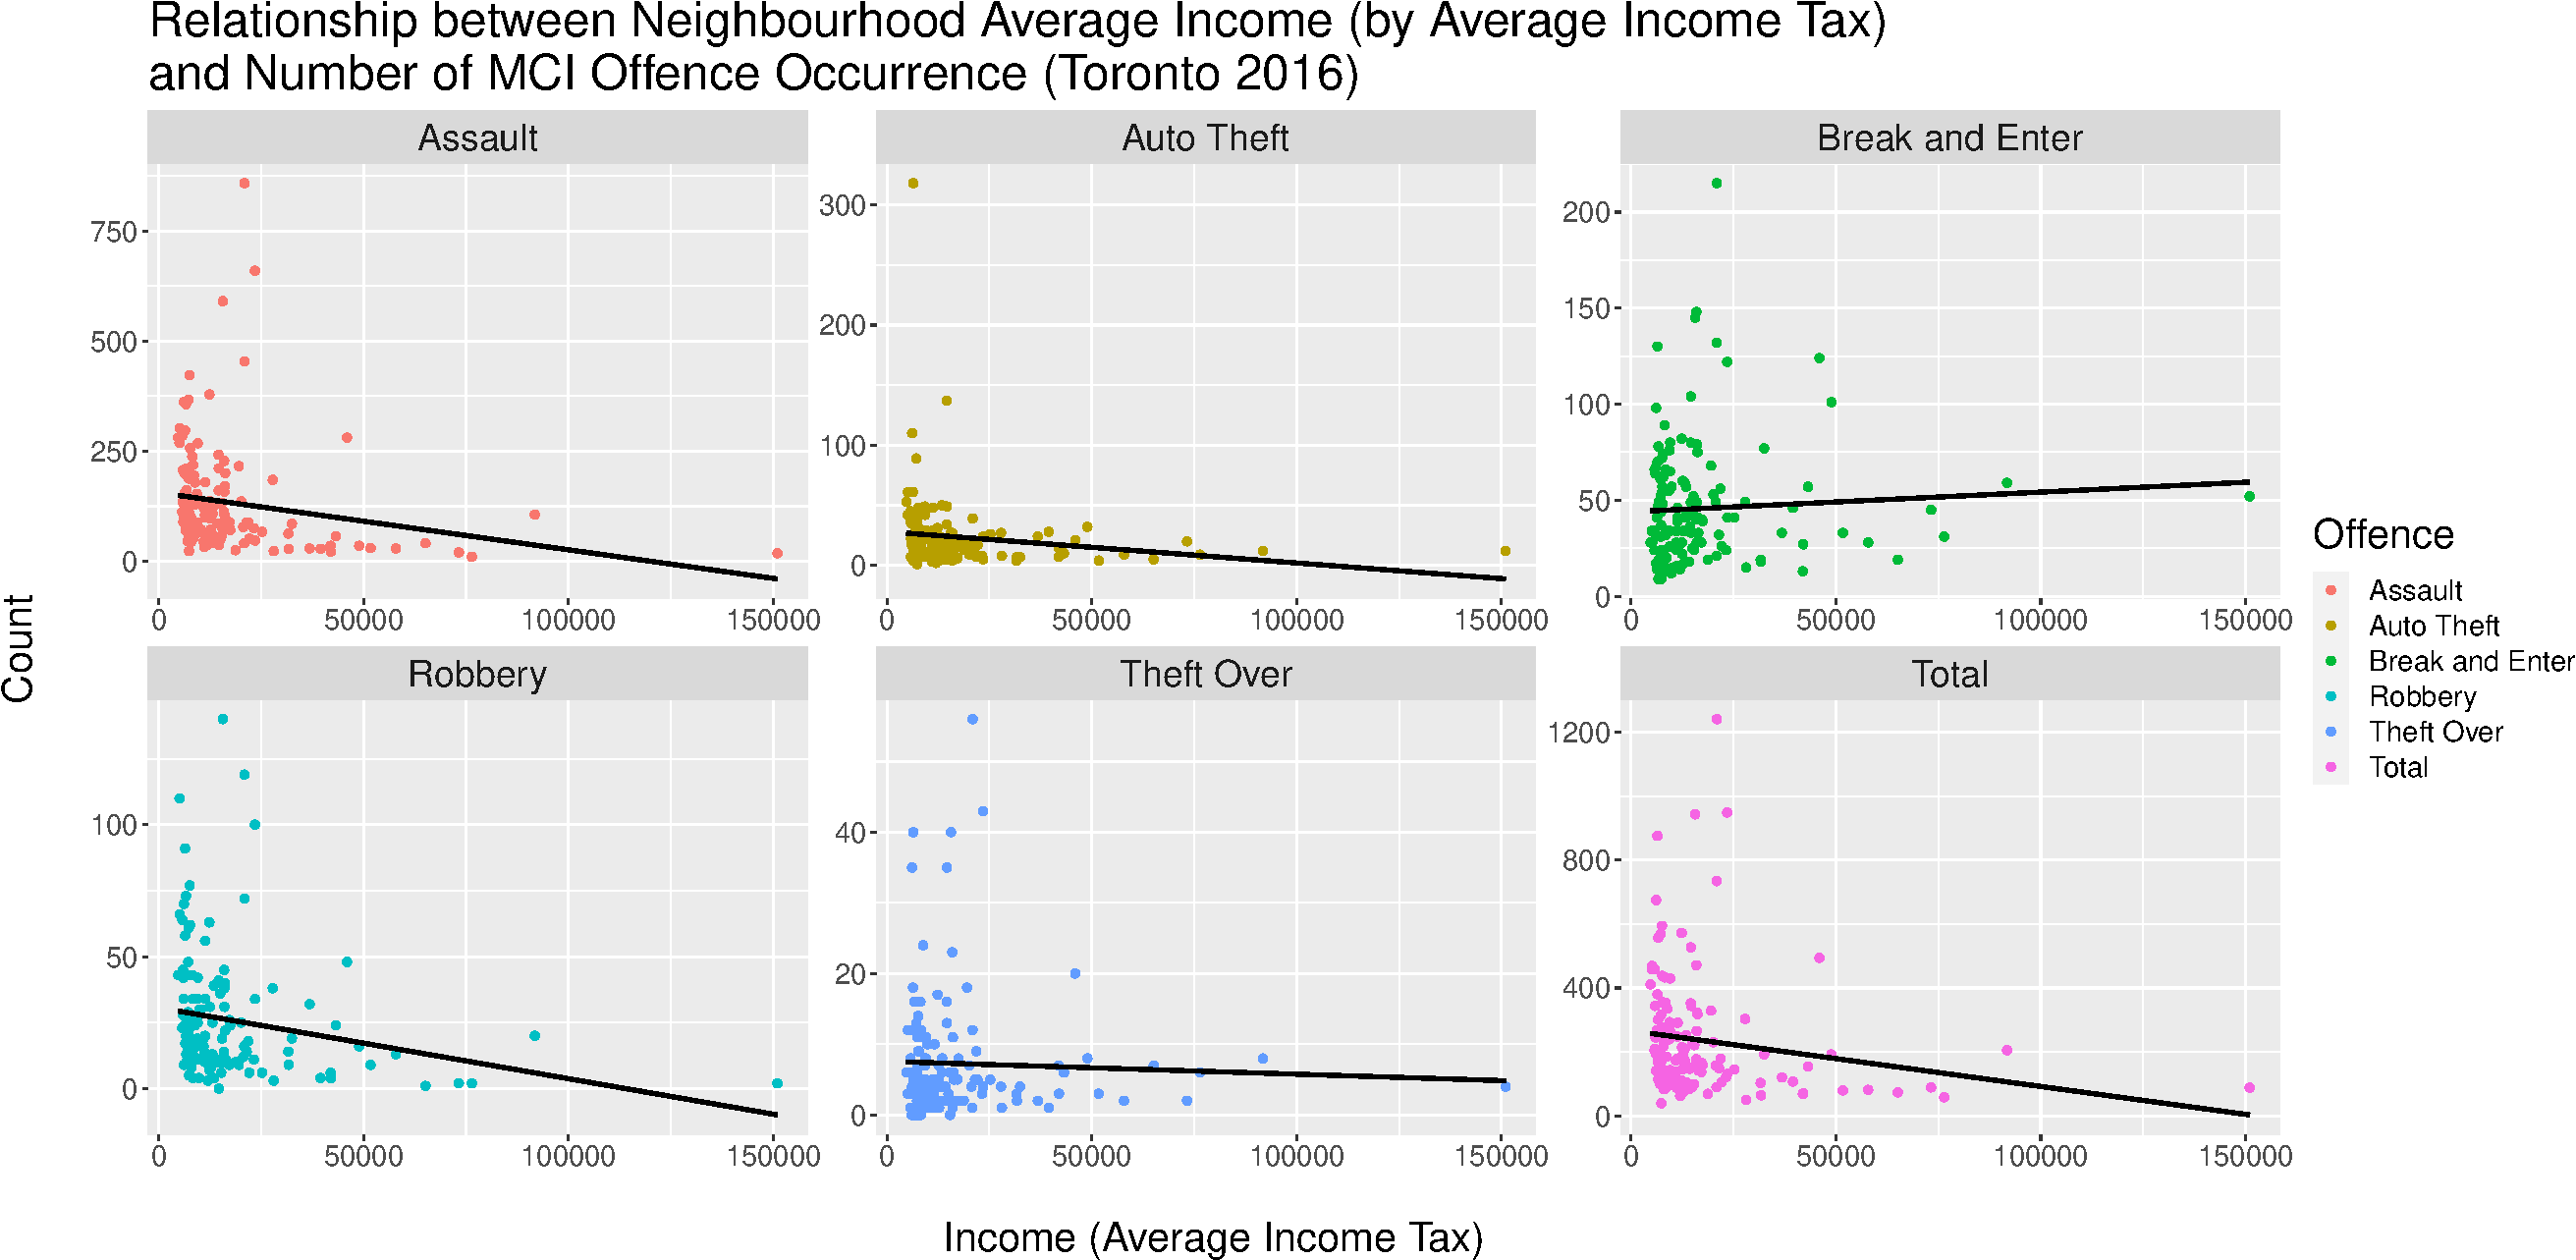
\includegraphics{Midterm-Report_files/figure-latex/crime-vs-income-plot-1.pdf}

\hypertarget{conclusions}{%
\section{Conclusions}\label{conclusions}}

In this report, we discussed how we performed exploratory data analysis
on how the demographics of a neighbourhood affected the crime rate of
the area in the 140 historical neighbourhoods in Toronto in 2016. Based
on prior research and some preliminary testing, we identified several
sigificant demographic factors which affected the number of offences
committed, including age, income, number of immigrants, level of
education, employment status and number of visible minorities in the
neighbourhood.

\hypertarget{limitations}{%
\section{Limitations}\label{limitations}}

There were several limitations in our research study.

First, in our preliminary testing plots and basic models, there were
many outliers and influential points in our predictor variables and
responses, which might have affected our interpretation of the results.
For example, in the plots of number of MCI offences against average
income tax, all the subplots showed a ``fanning pattern'', which meant
that the variance of the response were not Normally distributed and this
violation of linear model might affect the final result.

Second, the small amount of corrupted/mis-placed observations in the
``Neighbourhood Profiles'' dataset prevented us from using the income
groups directly to estimate the effect of average household and
individual income on neighbourhood crime rate. Instead, we utilised the
average income tax to represent the wealthiness of neighbourhoods.
Although income tax is positively correlated with individual and
household income, the data come in aggregated form (one number,
``average tax income'', for each neighbourhood), compared to the exact
numbers of individuals/household in each household. This reduced the
amount of information we could use and this could affect the final
result in our preliminary testing.

\hypertarget{next-steps}{%
\section{Next Steps}\label{next-steps}}

Despite the limitations above, most of our findings agreed with previous
researches, in that the variables of interest were significantly
correlated with neighbourhood crime rate. We could improved our existing
preliminary models by using a combination of different features as
predictors for predicting crime rate, in order to better explore the
interactions of these features and how they affected crime rate
together.

Another future step for this research could be to use the datasets to
build a predictive model on the number of MCI offences in the
neighbourhood, based on variables and features which are also correlated
with number of reported offence, such as the number of public spaces and
businesses, in addition to the demographic information we collected.
This, however, requires furthuer data collection.

\hypertarget{references}{%
\section{References}\label{references}}

\begin{enumerate}
\def\labelenumi{\arabic{enumi}.}
\item
  Foster, S., Giles-Corti, B., \& Knuiman, M. (2010). Neighbourhood
  design and fear of crime: A social-ecological examination of the
  correlates of residents' fear in new suburban housing developments. In
  Health \& Place (Vol. 16, Issue 6, pp.~1156--1165). Elsevier BV.
  \url{https://doi.org/10.1016/j.healthplace.2010.07.007}↩︎
\item
  Statistics Canada. (2021). Neighbourhood characteristics and life
  satisfaction of individuals in lower-, middle-, and higher-income
  families in Canadian metropolitan areas. Government of Canada.
  \url{https://doi.org/10.25318/36280001202100500006-ENG}↩︎
\item
  Government of Canada, S. C. (2020, July 17). Census of population.
  Surveys and statistical programs. Retrieved March 13, 2023, from
  \url{https://www23.statcan.gc.ca/imdb/p2SV.pl?Function=getSurvey\&SDDS=3901}↩︎
\item
  Statistics Canada. (n.d.). Main article. Neighbourhood Characteristics
  and the Distribution of Police-reported Crime in the City of Toronto.
  Retrieved March 13, 2023, from
  \url{https://www150.statcan.gc.ca/n1/pub/85-561-m/2009018/part-partie1-eng.htm}↩︎
\item
  Sun, Ivan Y.; Triplett, Ruth A.; and Gainey, Randy R., ``Neighborhood
  Characteristics and Crime: A Test of Sampson and Groves' Model of
  Social Disorganization'' (2004). Sociology \& Criminal Justice Faculty
  Publications. 3.
  \url{https://digitalcommons.odu.edu/sociology_criminaljustice_fac_pubs/3}↩︎
\item
  Ulmer, J. T., \& Steffensmeier, D. (2014). The age and crime
  relationship: Social variation, social explanations. In The Nurture
  Versus Biosocial Debate in Criminology: On the Origins of Criminal
  Behavior and Criminality (pp.~377-396). SAGE Publications Inc..
  \url{https://doi.org/10.4135/9781483349114.n23}↩︎
\item
  Farrington, D. P., Gallagher, B., Morley, L., St.~Ledger, R. J., \&
  West, D. J. (1986). UNEMPLOYMENT, SCHOOL LEAVING, AND CRIME. The
  British Journal of Criminology, 26(4), 335--356.
  \url{http://www.jstor.org/stable/23637076}↩︎
\item
  Kim, Y.-A., \& Wo, J. C. (2022, April 1). Racially diverse
  neighborhoods in diverse areas are linked to lower crime rates.
  Racially diverse neighborhoods in diverse areas are linked to lower
  crime rates Comments. Retrieved March 13, 2023, from
  \url{https://blogs.lse.ac.uk/usappblog/2022/04/01/racially-diverse-neighborhoods-in-diverse-areas-are-linked-to-lower-crime-rates/}
  ↩︎
\item
  Chamberlain, A. W., \& Boggess, L. N. (2016, September 26). Why
  disadvantaged neighborhoods are more attractive targets for burgling
  than wealthy ones. Why disadvantaged neighborhoods are more attractive
  targets for burgling than wealthy ones Comments. Retrieved March 13,
  2023, from
  \url{https://blogs.lse.ac.uk/usappblog/2016/09/26/why-disadvantaged-neighborhoods-are-more-attractive-targets-for-burgling-than-wealthy-ones/}↩︎
\end{enumerate}

\hypertarget{appendix}{%
\section{Appendix}\label{appendix}}

\hypertarget{table-1.-sample-of-dataset---major-crime-indicators}{%
\subsection{Table 1. Sample of Dataset - Major Crime
Indicators}\label{table-1.-sample-of-dataset---major-crime-indicators}}

\begin{longtable}{rllrrllrrlrlrrlrrlrrlrlrl}
\caption*{
{\large Major Crime Indicators} \\ 
{\small Occurrence of Crime from January 2014 to June 2022}
} \\ 
\toprule
X\_id & event\_unique\_id & Division & occurrencedate & reporteddate & location\_type & premises\_type & ucr\_code & ucr\_ext & offence & reportedyear & reportedmonth & reportedday & reporteddayofyear & reporteddayofweek & reportedhour & occurrenceyear & occurrencemonth & occurrenceday & occurrencedayofyear & occurrencedayofweek & occurrencehour & mci\_category & Hood\_ID & Neighbourhood \\ 
\midrule
1 & GO-20141273318 & D31 & 2014-01-03 & 2014-01-03 & Apartment (Rooming House, Condo) & Apartment & 1430 & 100 & Assault & 2014 & January & 3 & 3 & Friday     & 11 & 2014 & January & 3 & 3 & Friday     & 11 & Assault & 27 & York University Heights \\ 
2 & GO-20141274349 & D42 & 2014-01-03 & 2014-01-03 & Single Home, House (Attach Garage, Cottage, Mobile) & House & 2120 & 200 & B\&E & 2014 & January & 3 & 3 & Friday     & 14 & 2014 & January & 3 & 3 & Friday     & 14 & Break and Enter & 132 & Malvern \\ 
3 & GO-20141274052 & D22 & 2014-01-03 & 2014-01-03 & Open Areas (Lakes, Parks, Rivers) & Outside & 1430 & 100 & Assault & 2014 & January & 3 & 3 & Friday     & 13 & 2014 & January & 3 & 3 & Friday     & 13 & Assault & 19 & Long Branch \\ 
4 & GO-20141276966 & D53 & 2014-01-03 & 2014-01-03 & Other Commercial / Corporate Places (For Profit, Warehouse, Corp. Bldg & Commercial & 2130 & 210 & Theft Over & 2014 & January & 3 & 3 & Friday     & 13 & 2014 & January & 3 & 3 & Friday     & 12 & Theft Over & 55 & Thorncliffe Park \\ 
\bottomrule
\end{longtable}

\hypertarget{table-2.-sample-of-dataset---neighbourhood-profiles-census}{%
\subsection{Table 2. Sample of Dataset - Neighbourhood Profiles
(Census)}\label{table-2.-sample-of-dataset---neighbourhood-profiles-census}}

\begin{longtable}{rllllrllllllllllllllllllllllllllllllllllllllllllllllllllllllllllllllllllllllllllllllllllllllllllllllllllllllllllllllllllllllllllllllllllllllllllll}
\caption*{
{\large Neighbourhood Profiles} \\ 
{\small Census of Neighbourhoods in 2016}
} \\ 
\toprule
X\_id & Category & Topic & Data.Source & Characteristic & City.of.Toronto & Agincourt.North & Agincourt.South.Malvern.West & Alderwood & Annex & Banbury.Don.Mills & Bathurst.Manor & Bay.Street.Corridor & Bayview.Village & Bayview.Woods.Steeles & Bedford.Park.Nortown & Beechborough.Greenbrook & Bendale & Birchcliffe.Cliffside & Black.Creek & Blake.Jones & Briar.Hill.Belgravia & Bridle.Path.Sunnybrook.York.Mills & Broadview.North & Brookhaven.Amesbury & Cabbagetown.South.St..James.Town & Caledonia.Fairbank & Casa.Loma & Centennial.Scarborough & Church.Yonge.Corridor & Clairlea.Birchmount & Clanton.Park & Cliffcrest & Corso.Italia.Davenport & Danforth & Danforth.East.York & Don.Valley.Village & Dorset.Park & Dovercourt.Wallace.Emerson.Junction & Downsview.Roding.CFB & Dufferin.Grove & East.End.Danforth & Edenbridge.Humber.Valley & Eglinton.East & Elms.Old.Rexdale & Englemount.Lawrence & Eringate.Centennial.West.Deane & Etobicoke.West.Mall & Flemingdon.Park & Forest.Hill.North & Forest.Hill.South & Glenfield.Jane.Heights & Greenwood.Coxwell & Guildwood & Henry.Farm & High.Park.North & High.Park.Swansea & Highland.Creek & Hillcrest.Village & Humber.Heights.Westmount & Humber.Summit & Humbermede & Humewood.Cedarvale & Ionview & Islington.City.Centre.West & Junction.Area & Keelesdale.Eglinton.West & Kennedy.Park & Kensington.Chinatown & Kingsview.Village.The.Westway & Kingsway.South & Lambton.Baby.Point & L.Amoreaux & Lansing.Westgate & Lawrence.Park.North & Lawrence.Park.South & Leaside.Bennington & Little.Portugal & Long.Branch & Malvern & Maple.Leaf & Markland.Wood & Milliken & Mimico..includes.Humber.Bay.Shores. & Morningside & Moss.Park & Mount.Dennis & Mount.Olive.Silverstone.Jamestown & Mount.Pleasant.East & Mount.Pleasant.West & New.Toronto & Newtonbrook.East & Newtonbrook.West & Niagara & North.Riverdale & North.St..James.Town & Oakridge & Oakwood.Village & O.Connor.Parkview & Old.East.York & Palmerston.Little.Italy & Parkwoods.Donalda & Pelmo.Park.Humberlea & Playter.Estates.Danforth & Pleasant.View & Princess.Rosethorn & Regent.Park & Rexdale.Kipling & Rockcliffe.Smythe & Roncesvalles & Rosedale.Moore.Park & Rouge & Runnymede.Bloor.West.Village & Rustic & Scarborough.Village & South.Parkdale & South.Riverdale & St.Andrew.Windfields & Steeles & Stonegate.Queensway & Tam.O.Shanter.Sullivan & Taylor.Massey & The.Beaches & Thistletown.Beaumond.Heights & Thorncliffe.Park & Trinity.Bellwoods & University & Victoria.Village & Waterfront.Communities.The.Island & West.Hill & West.Humber.Clairville & Westminster.Branson & Weston & Weston.Pelham.Park & Wexford.Maryvale & Willowdale.East & Willowdale.West & Willowridge.Martingrove.Richview & Woburn & Woodbine.Corridor & Woodbine.Lumsden & Wychwood & Yonge.Eglinton & Yonge.St.Clair & York.University.Heights & Yorkdale.Glen.Park \\ 
\midrule
1 & Neighbourhood Information & Neighbourhood Information & City of Toronto & Neighbourhood Number &  & 129 & 128 & 20 & 95 & 42 & 34 & 76 & 52 & 49 & 39 & 112 & 127 & 122 & 24 & 69 & 108 & 41 & 57 & 30 & 71 & 109 & 96 & 133 & 75 & 120 & 33 & 123 & 92 & 66 & 59 & 47 & 126 & 93 & 26 & 83 & 62 & 9 & 138 & 5 & 32 & 11 & 13 & 44 & 102 & 101 & 25 & 65 & 140 & 53 & 88 & 87 & 134 & 48 & 8 & 21 & 22 & 106 & 125 & 14 & 90 & 110 & 124 & 78 & 6 & 15 & 114 & 117 & 38 & 105 & 103 & 56 & 84 & 19 & 132 & 29 & 12 & 130 & 17 & 135 & 73 & 115 & 2 & 99 & 104 & 18 & 50 & 36 & 82 & 68 & 74 & 121 & 107 & 54 & 58 & 80 & 45 & 23 & 67 & 46 & 10 & 72 & 4 & 111 & 86 & 98 & 131 & 89 & 28 & 139 & 85 & 70 & 40 & 116 & 16 & 118 & 61 & 63 & 3 & 55 & 81 & 79 & 43 & 77 & 136 & 1 & 35 & 113 & 91 & 119 & 51 & 37 & 7 & 137 & 64 & 60 & 94 & 100 & 97 & 27 & 31 \\ 
2 & Neighbourhood Information & Neighbourhood Information & City of Toronto & TSNS2020 Designation &  & No Designation & No Designation & No Designation & No Designation & No Designation & No Designation & No Designation & No Designation & No Designation & No Designation & NIA & No Designation & No Designation & NIA & No Designation & No Designation & No Designation & No Designation & No Designation & No Designation & No Designation & No Designation & No Designation & No Designation & No Designation & No Designation & No Designation & No Designation & No Designation & No Designation & No Designation & Emerging Neighbourhood & No Designation & NIA & No Designation & No Designation & No Designation & NIA & NIA & Emerging Neighbourhood & No Designation & No Designation & NIA & No Designation & No Designation & NIA & No Designation & No Designation & No Designation & No Designation & No Designation & No Designation & No Designation & Emerging Neighbourhood & NIA & NIA & No Designation & NIA & No Designation & No Designation & NIA & NIA & No Designation & NIA & No Designation & No Designation & Emerging Neighbourhood & No Designation & No Designation & No Designation & No Designation & No Designation & No Designation & Emerging Neighbourhood & No Designation & No Designation & No Designation & No Designation & NIA & No Designation & NIA & NIA & No Designation & No Designation & No Designation & No Designation & No Designation & No Designation & No Designation & No Designation & NIA & No Designation & No Designation & No Designation & No Designation & No Designation & No Designation & No Designation & No Designation & No Designation & NIA & No Designation & NIA & No Designation & No Designation & No Designation & No Designation & NIA & NIA & NIA & No Designation & No Designation & Emerging Neighbourhood & No Designation & No Designation & NIA & No Designation & NIA & NIA & No Designation & No Designation & NIA & No Designation & NIA & No Designation & Emerging Neighbourhood & NIA & NIA & No Designation & No Designation & No Designation & No Designation & NIA & No Designation & No Designation & No Designation & No Designation & No Designation & NIA & Emerging Neighbourhood \\ 
3 & Population & Population and dwellings & Census Profile 98-316-X2016001 & Population, 2016 & 2,731,571 & 29,113 & 23,757 & 12,054 & 30,526 & 27,695 & 15,873 & 25,797 & 21,396 & 13,154 & 23,236 & 6,577 & 29,960 & 22,291 & 21,737 & 7,727 & 14,257 & 9,266 & 11,499 & 17,757 & 11,669 & 9,955 & 10,968 & 13,362 & 31,340 & 26,984 & 16,472 & 15,935 & 14,133 & 9,666 & 17,180 & 27,051 & 25,003 & 36,625 & 35,052 & 11,785 & 21,381 & 15,535 & 22,776 & 9,456 & 22,372 & 18,588 & 11,848 & 21,933 & 12,806 & 10,732 & 30,491 & 14,417 & 9,917 & 15,723 & 22,162 & 23,925 & 12,494 & 16,934 & 10,948 & 12,416 & 15,545 & 14,365 & 13,641 & 43,965 & 14,366 & 11,058 & 17,123 & 17,945 & 22,000 & 9,271 & 7,985 & 43,993 & 16,164 & 14,607 & 15,179 & 16,828 & 15,559 & 10,084 & 43,794 & 10,111 & 10,554 & 26,572 & 33,964 & 17,455 & 20,506 & 13,593 & 32,954 & 16,775 & 29,658 & 11,463 & 16,097 & 23,831 & 31,180 & 11,916 & 18,615 & 13,845 & 21,210 & 18,675 & 9,233 & 13,826 & 34,805 & 10,722 & 7,804 & 15,818 & 11,051 & 10,803 & 10,529 & 22,246 & 14,974 & 20,923 & 46,496 & 10,070 & 9,941 & 16,724 & 21,849 & 27,876 & 17,812 & 24,623 & 25,051 & 27,446 & 15,683 & 21,567 & 10,360 & 21,108 & 16,556 & 7,607 & 17,510 & 65,913 & 27,392 & 33,312 & 26,274 & 17,992 & 11,098 & 27,917 & 50,434 & 16,936 & 22,156 & 53,485 & 12,541 & 7,865 & 14,349 & 11,817 & 12,528 & 27,593 & 14,804 \\ 
4 & Population & Population and dwellings & Census Profile 98-316-X2016001 & Population, 2011 & 2,615,060 & 30,279 & 21,988 & 11,904 & 29,177 & 26,918 & 15,434 & 19,348 & 17,671 & 13,530 & 23,185 & 6,488 & 27,876 & 21,856 & 22,057 & 7,763 & 14,302 & 8,713 & 11,563 & 17,787 & 12,053 & 9,851 & 10,487 & 13,093 & 28,349 & 24,770 & 14,612 & 15,703 & 13,743 & 9,444 & 16,712 & 26,739 & 24,363 & 34,631 & 34,659 & 11,449 & 20,839 & 14,943 & 22,829 & 9,550 & 22,086 & 18,810 & 10,927 & 22,168 & 12,474 & 10,926 & 31,390 & 14,083 & 9,816 & 11,333 & 21,292 & 21,740 & 13,097 & 17,656 & 10,583 & 12,525 & 15,853 & 14,108 & 13,091 & 38,084 & 14,027 & 10,638 & 17,058 & 18,495 & 21,723 & 9,170 & 7,921 & 44,919 & 14,642 & 14,541 & 15,070 & 17,011 & 12,050 & 9,632 & 45,086 & 10,197 & 10,436 & 27,167 & 26,541 & 17,587 & 16,306 & 13,145 & 32,788 & 15,982 & 28,593 & 10,900 & 16,423 & 23,052 & 21,274 & 12,191 & 17,832 & 13,497 & 21,073 & 18,316 & 9,118 & 13,746 & 34,617 & 8,710 & 7,653 & 16,144 & 11,197 & 10,007 & 10,488 & 22,267 & 15,050 & 20,631 & 45,912 & 9,632 & 9,951 & 16,609 & 21,251 & 25,642 & 17,958 & 25,017 & 24,691 & 27,398 & 15,594 & 21,130 & 10,138 & 19,225 & 16,802 & 7,782 & 17,182 & 43,361 & 26,547 & 34,100 & 25,446 & 18,170 & 12,010 & 27,018 & 45,041 & 15,004 & 21,343 & 53,350 & 11,703 & 7,826 & 13,986 & 10,578 & 11,652 & 27,713 & 14,687 \\ 
\bottomrule
\end{longtable}

\hypertarget{table-3.-sample-of-cleaned-dataset---major-crime-indicators}{%
\subsection{Table 3. Sample of Cleaned Dataset - Major Crime
Indicators}\label{table-3.-sample-of-cleaned-dataset---major-crime-indicators}}

\begin{longtable}{rrlllrlrrlrrlrrlrlrl}
\caption*{
{\large Major Crime Indicators (2016)} \\ 
{\small Occurrence of Crime in 2016}
} \\ 
\toprule
occurrencedate & reporteddate & location\_type & premises\_type & offence & reportedyear & reportedmonth & reportedday & reporteddayofyear & reporteddayofweek & reportedhour & occurrenceyear & occurrencemonth & occurrenceday & occurrencedayofyear & occurrencedayofweek & occurrencehour & mci\_category & Hood\_ID & Neighbourhood \\ 
\midrule
2016-01-01 & 2016-01-01 & Apartment (Rooming House, Condo) & Apartment & Assault With Weapon & 2016 & January & 1 & 1 & Friday     & 3 & 2016 & January & 1 & 1 & Friday     & 3 & Assault & 70 & South Riverdale \\ 
2016-01-06 & 2016-01-06 & Single Home, House (Attach Garage, Cottage, Mobile) & House & B\&E & 2016 & January & 6 & 6 & Wednesday  & 13 & 2016 & January & 6 & 6 & Wednesday  & 13 & Break and Enter & 86 & Roncesvalles \\ 
2016-01-01 & 2016-01-01 & Single Home, House (Attach Garage, Cottage, Mobile) & House & Assault With Weapon & 2016 & January & 1 & 1 & Friday     & 4 & 2016 & January & 1 & 1 & Friday     & 3 & Assault & 31 & Yorkdale-Glen Park \\ 
2016-01-06 & 2016-01-06 & Streets, Roads, Highways (Bicycle Path, Private Road) & Outside & Robbery - Mugging & 2016 & January & 6 & 6 & Wednesday  & 12 & 2016 & January & 6 & 6 & Wednesday  & 12 & Robbery & 101 & Forest Hill South \\ 
\bottomrule
\end{longtable}

\end{document}
